\documentclass[openbib,12pt]{article}  % Comments shown
\usepackage{linlib}
\usepackage{lawreview}

\usepackage{amsmath,amssymb,amsthm,mathabx}
\usepackage{amsfonts}
\usepackage{amsmath}
\usepackage{amssymb}
\usepackage{makeidx}
\usepackage{arydshln}
\usepackage{natbib}
%\usepackage[utf8x]{inputenc}
%\usepackage[colorinlistoftodos]{todonotes}
%\usepackage[margin=1in]{geometry}
\usepackage{mathpazo}
%\usepackage{dsfont}
\usepackage[multiple]{footmisc}
\usepackage{graphicx}
\usepackage{setspace}
\usepackage{booktabs}
%\usepackage[colorlinks,citecolor=blue]{hyperref}
\usepackage[hidelinks]{hyperref}
\usepackage{lscape}
\usepackage[hang,centerlast]{caption}
%\usepackage{makecell}
\usepackage{multirow}
%\usepackage[flushleft]{threeparttable}
\usepackage[pdftex]{color}
\usepackage[table]{xcolor}
\usepackage{rotating}
\usepackage{url}
\usepackage{tikz}
\usetikzlibrary{arrows, intersections, patterns}
\usepackage{pgfplots}
\pgfplotsset{compat=newest}
\usepgfplotslibrary{fillbetween}
% We will externalize the figures
\usepgfplotslibrary{external}
\usepackage{environ}
\tikzexternalize[prefix=figures/]
%\tikzset{external/optimize=false}
\usetikzlibrary{calc}
\usetikzlibrary{positioning}
\usetikzlibrary{intersections}%, pgfplots.fillbetween}
\usetikzlibrary{patterns}
\usepgfplotslibrary{fillbetween}
\usepackage{subfigure}
\usepackage[capposition=bottom]{floatrow}
\usepackage[all]{xy}
\usepackage[english]{babel}
\usepackage{adjustbox}
\DeclareGraphicsRule{*}{mps}{*}{}
\newtheorem{assumption}{Assumption}
\newtheorem{claim}{Claim}
\newtheorem{example}{Example}
\newtheorem{definition}{Definition}
\newtheorem{lemma}{Lemma}
\newtheorem{proposition}{Proposition}
\newtheorem{theorem}{Theorem}
\newtheorem{corollary}{Corollary}
\newtheorem{hypothesis}{Hypothesis}
\newtheorem{result}{Result}
\newtheorem{finding}{Finding}
\newtheorem{subfinding}{Finding}
\renewcommand{\thesubfinding}{\thefinding\alph{subfinding}}
\newtheorem{subhypothesis}{Hypothesis}
\renewcommand{\thesubhypothesis}{\thehypothesis\alph{subhypothesis}}
\newcommand{\argmax}{\operatornamewithlimits{argmax}}
\newcommand{\supp}{\operatorname{supp}}
\newcommand{\Var}{\mathrm{Var}}
\newcommand{\Cov}{\mathrm{Cov}}
\newcommand{\plim}{\mathrm{plim}}
\newcommand{\tred}{\textcolor{red}}
\newcommand{\lmt}{\rightarrow}
\newcommand{\lmp}{\Rightarrow}
\newcommand{\lt}{\left}
\newcommand{\rt}{\right}
\newcommand{\nn}{\nonumber}
\newcommand{\gs}{\geqslant}
\newcommand{\ls}{\leqslant}
%% specific to this paper

%\renewcommand{\baselinestretch}{1.4} 
\renewcommand{\vec}[1]{\mathbf{#1}}
% \oddsidemargin=0truein
% \evensidemargin=0truein
% \topmargin=0truein\headheight=0truein\headsep=0truein
% \textheight=9truein\textwidth=6.5truein
% \parskip=12pt
% \parindent=1cm
% \baselineskip=25pt

\title{An Economic Model of Intermediary Liability}
\author{James Grimmelmann\footnote{Cornell Law School and Cornell Tech, Cornell University, james.grimmelmann@cornell.edu}
\and Pengfei Zhang\footnote{School of Economic, Political and Policy Sciences, The University of Texas at Dallas, pengfei.zhang@utdallas.edu}}
\date{June 2021}

\begin{document}

\maketitle
\begin{abstract}
\noindent 
% This paper presents an economic analysis of intermediary liability. We develop a simple model of a platform's trade-off to moderate content, and use the model to analyze five liability rules on the intermediary: immunity, strict liability, free speech, safe harbor, and liability upon notice. The efficiency of the legal rules depends upon the social benefit of content and the platform's information regarding harm. 
% When the platform has perfect information on the harm and its content imposes no externalities on society, all the liability rules except immunity are efficient. Intermediary immunity is efficient only if the positive externality of content is sufficiently strong. However, with imperfect information and positive externalities, none of the rules is efficient, but a safe harbor conditional on a threshold of screening effort might lead to an efficient outcome.
In the debates about intermediary liability, numerous scholars have given informal economic arguments about the costs and benefits of different liability rules. Some scholars, for example, have argued that broad immunity is justified because platforms fail to internalize the social benefits of the content they carry -- so that strict liability predictably results in overmoderation. Others, however, have claimed that platforms fail to internalize the social harms of the content they carry -- so that blanket immunity predictably results in undermoderation.

In this paper, we seek to illuminate these debates by giving a more formal economic model of intermediary liability. The key feature of our model is \emph{imperfect information}: the platform observes the probability that each item of content is harmful, and can choose to take the content down, leave it up, or incur a cost to determine with certainty whether the content is harmful. The platform's choice reflects the tradeoffs inherent in content moderation: between false positives and false negatives, and between scalable but more error-prone processes and more intensive but costly human review. We analyze various plausible legal regimes, including strict liability, blanket immunity, negligence, reasonable efforts, liability on notice, and must-carry, and we use them to describe current and proposed laws in the United States and European Union.


\vspace{0in}
%\noindent\textbf{Keywords:} Intermediary Liability, Content Moderation, Section 230, Digital Platform, Externalities, Imperfect Information \\
%\vspace{0in}\\
%\noindent\textbf{JEL Codes:} D74, K13, K24, L51.\\
% if, when, with, for, there is no
%\bigskip
\end{abstract}

\newpage
\tableofcontents

\newpage

\section{Introduction}\label{EMIL_Section:intro}
In the scholarly literature on intermediary liability, economic claims are common. Here are a few:

\begin{itemize}
\item t/k
\end{itemize}

These claims are common, but they are mostly informal. They are policy arguments, not testable propositions. It is not clear when two claims conflict, or when they can coexist. Indeed, it is often not even clear whether two authors are making the same claim, or different claims.

We do not propose to resolve any of these disputes. Instead, we aim to clarify the terms of the debate. In this paper, we recast arguments about intermediary liability into a common language -- the language of microeconomics. We give an economic model of intermediary liability, with equations and diagrams. We see six signifiant benefits from having such a model.

First and most fundamentally, modeling promotes communication. A suitable model can serve as a common framework for scholars to compare and contrast arguments. Our taxonomy of liability regimes reduces the at-times bewildering array of arguments about the proper scope of intermediary liability into a (we hope) orderly structure that makes it straightforward to see how different claims relate.

Second, modeling promotes intuition. A good model can bring out the consequences of a course of conduct, or make plain why parties behave the way that they do. There are several common patterns in intermediary-liability law that have simple and vivid expressions in our model.

Third, modeling promotes visualization. We have attempted to provide a simple and memorable visual shorthand for every moving part in our model and every interesting effect of a legal regime. For example, we hope that even you take nothing else away from this paper, you will have a clear visual sense for why a platform might either overmoderate or undermoderate even in the absence of liability.

Fourth, modeling promotes rigor. The process of writing down a model forces one to make implicit assumptions explicit. The process of reasoning through a model's consequences forces one to examine each claimed effect closely. In the course of working through our own model, we learned a lot about how arguments for and against intermediary immunity work, and this paper conveys some of what we have learned.

Fifth, modeling promotes proof. Given a set of assumptions, it is possible to show rigorously that particular conclusions follow. We demonstrate, for example, that under our assumptions, strict liability consistently results in overmoderation. Of course, the real world is not required to comply with a proof about a model. But proofs like these make models more useful, because they help pin down the predictions the model actually makes.

And sixth, modeling promotes empiricism. This is not an econometric paper; it uses no datasets and very few numbers. But a model like ours helps pin down which econometric questions to ask. We hope that it provides a roadmap for future empirical work.

This paper has four Parts, not counting this introduction and a brief conclusion. Part \ref{sect:prior} describes the limited previous work in this space. Part \ref{sect:model} describes the model in formal detail. Part \ref{sect:liability} analyzes a variety of liability regimes in detail. And Part \ref{sect:laws} shows how various current and proposed laws map on to those liability regimes.

\section{Background and Related Literature}\label{EMIL_Section:inst}
\label{sec:background}



Economic models of liability start from the pioneering work of \cite{brown1973toward} and are further developed by many important contributions, including \cite{shavell1980strict}, which are summarized in \cite{shavell2009accident}. 
In the economic analysis, the goal of the liability system is to promote efficiency, which means minimizing the total social costs.  
The focus is on the effect of different liability rules, mainly strict liability and the negligence rule, on incentives for taking precaution to reduce risk. 
One of the key insights is that if only injurers influence risks, both strict liability and the negligence rule can induce the injurers to take optimal care.  

% injurers are firms
The economic theory of liability extends to the case of product liability where a manufacturer or seller might be held liable for harm caused by a defective or unsafe product. 
This requires us to take into account the relationship between liability, market price, and the profit-maximizing production of the firms. 
Important contributions include \cite{hamada1976liability}, \cite{polinsky1980strict}, \cite{landes1985positive}, \cite{polinsky2010uneasy}, and \cite{daughety2013economic} provides an excellent review. 
One of the key insights of this literature is whether and how to impose liability depends on the characteristics of the product and the information of the consumers.  
For example, a strict liability rule would be more appropriate when it is difficult to test for product safety.
In general, strict liability is more efficient than the negligence rule, as it either results in prices that induce optimal production or induces consumers to purchase the optimal quantity. 

Economic literature on intermediary liability, however, is still at its infancy stage.  
\cite{hua2021holding} extends the product liability framework to a two-sided platform that enables interactions between sellers and buyers. By either raising price or investing in screening, the platform wants to keep the safe sellers while deterring the harmful sellers. The authors argue that whether to impose liability on the platform is a judgement proof problem. If the sellers have deep pocket then intermediary immunity is optimal. If instead the sellers are judgement proof, then intermediary liability is necessary and imposing the residual liability on the platform improves social welfare.  
\cite{buiten2020rethinking} examine the liability of online hosting platforms for user-generated content, specifically in the context of the European Union's Digital Single Market strategy. They argue that the current EU liability framework is outdated and inadequate for dealing with the challenges of online content moderation. The absence of ``Good Samaritan'' protection in the EU e-Commerce Directive creates perverse incentives for platforms not to monitor online activity, thus undermining self-regulation. 
They propose a three-tiered approach, in which platforms are responsible for different types of content depending on their level of control over the content. 
This literature so far focus on comparing intermediary immunity with strict liability. In this paper, we also examines alternative liability rules that are popular in the legal debate, including negligence, must-carry rule, liability upon notice, and safe harbor. 


%\section{Law Review Model}\label{EMIL_Section:lawreview}

% TikZ macros
\usetikzlibrary{arrows.meta, intersections, patterns}

\newenvironment{econ}[2]
{
  \begin{figure}[h]
	  \centering
  %\caption{#1}
  \label{#2}
  \begin{tikzpicture}[scale=1]
}
{
  \end{tikzpicture}
  \end{figure}
}

\newenvironment{pgfecon}[2]
{
  \begin{figure}[h]
  \centering
  \caption{#1}
  \label{#2}
  \begin{tikzpicture}[scale=1]
  \begin{axis}[
	  axis lines* = middle,
	  xmin = -.2,
	  xmax = 10,
	  width=12cm,
	  ymin = -1,
	  ymax = 6,
	  height=8cm,
	  xtick=\empty,
	  ytick=\empty,
	  clip=false
  ]
  \path[name path=axis] (0,0) -- (10,0);
}
{
  \end{axis}
  \end{tikzpicture}
  \end{figure}
}



\newcommand{\drawaxes}[2] { 
	\draw[name path = xaxis, -|] (-0.2,0) -- (10,0) node[below]{}; 
	\draw[name path = yaxis, ->] (0,-0.2) -- (0,5.5) node[left]{} ;
}


\newcommand{\harmplot} {
  \addplot [-, name path = harmline,
  domain = 0:10,
  samples = 250] {5}
  node[very near start, above]{$H$};
}

\newcommand{\scurveplot}[1] {
  \addplot [-, name path = lambda, thick,
  domain = 0:10,
  samples = 250] { \x < 1 ? 0 : 
        (\x < 5 ? (\x - 1)^ 2 / 6.4 : 
        (\x < 9 ? 5 - (9-\x)^2 / 6.4  :
        5
        ))}  node[right]{#1};
}

\newcommand{\hplot}{\scurveplot{$h(x)$}}

\newcommand{\lambdaplot} {\scurveplot{$H\lambda(x)$}}

\newcommand{\lambdaline} {
 \addplot [-, name path = lambda, thick, domain = 0:10, samples = 250] { \x /2 )}  node[right]{$H\lambda(x)$};
}


\newcommand{\testplot}[1] {
\addplot [-, name path = profit, thick,
domain = 0:10,
samples = 250] {#1}
node[very near end, left]{$t(x)$};
}
\newcommand{\profitplot} {
 \addplot [-, name path = profit, thick,
domain = 0:10,
samples = 250] { \x < 1.5 ? 2.5 : 
				  (\x < 6.5 ? 2.5 - (\x - 1.5)^2 / 15 : 
				  .8333 - (\x - 6.5) / 1.625)}
node[very near end, left]{$p(x)$};
}

\newcommand{\welfareplot} {
 \addplot [-, name path = profit, thick,
domain = 0:10,
samples = 250] { \x < 1.5 ? 3.5 : 
				  (\x < 6.5 ? 3.5 - (\x - 1.5)^2 / 18 : 
				  2.111 - (\x - 6.5) / 1.875)}
node[very near end, above]{$s(x)$};
}


\newcommand{\plotline}[3] {
\addplot [-, name path = #1, dotted,
domain = 0:10,
samples = 250] {#2}
node[at start, left]{#3};
}

\newcommand{\plotvalue}[4] {
\addplot [-, name path = #1, thick,
domain = 0:10,
samples = 250] {
   \x < 1.5 ? #2 : 
   (\x < 6.5 ? #2 - (\x - 1.5)^2 / #3 : 
   #2 - (25 / #3) - (10 * (\x - 6.5)) / #3 }
node[right]{#4};
}

\newcommand{\plotpartialvalue}[5] {
\addplot [-, thick, color=#5,
domain = #3:#4,
samples = 250] {
 \x < 1.5 ? #1 : 
 (\x < 6.5 ? #1 - (\x - 1.5)^2 / #2 : 
 #1 - (25 / #2) - (10 * (\x - 6.5)) / #2 }
}

\newcommand{\harmfunction}[1] {
	\draw[name path=harm, thick] (0,0) to (1,0) parabola (5,2.5) parabola[bend at end] (9,5) to (10,5) node[right]{#1};
}

\newcommand{\harmline}[1] {
	\draw[name path=harm, thick] (0,5) -- node[above]{#1} (10,5);
}

\newcommand{\revenueline}[1] {
	\draw[name path=revenue, thick] (0,1.5) to (10,1.5) node[right]{#1};
}

\newcommand{\revenuecurve}[1] {
	\draw [name path=revenue] (0,3) to (2, 3) parabola (6,1.75) to (10, -1) node[right]{#1};
}

\newcommand{\dropline}[3]{
  \draw[dashed, thin] (#1, #2) -- (#1, 0) node[below]{#3};
}

\newcommand{\xe} {
	\draw[dashed, thin] (4.1,1.5) -- (4.1,0) node[below]{$x^e$}; 
}

\newcommand{\xexhat} {
	\draw[dashed, thin] (4.1,1.5) -- (4.1,0) node[below]{$\hat{x} = x^e$}; 
}


\newcommand{\xhat}[1]{
   \draw[dashed, thin] (#1,1.5) -- (#1,0) node[below]{$\hat{x}$}; 
}

\newcommand{\spilloverfunction}[1] {
	  \draw [name path=welfare] (0,4.25) to (2, 4.25) parabola (6,3) to (10, 0.25) node[right]{#1};
}

\newcommand{\spilloverline}[1] {
	\draw[thick] (0,2.5) to (10,2.5) node[right]{#1};
}

% \NewDocumentCommand\drawarrows{O{0.5}mmO{-latex}mm}{
% \def\Step{#1}
% \pgfmathsetmacro{\Second}{#5+\Step}
% \foreach \Value [count=\xi] in {#5,\Second,...,#6}
%   {
%   \path[overlay,name path=line\xi] 
%     (\Value,100) -- (\Value,-100);
%   \path[name intersections={of=#2 and line\xi,by={1\xi}}];
%   \path[name intersections={of=#3 and line\xi,by={2\xi}}];
%   \ifdim#5pt<\Value pt\relax
%     \ifdim\Value pt<#6pt\relax
%     \draw[#4]
%       (1\xi) -- (2\xi); 
%   \fi\fi
%   }
%  }

\newcommand{\xmax}{x_{\text{max}}}
\newcommand{\xbi}{x_{\text{BI}}^*}
\newcommand{\xsl}{x_{\text{SL}}^*}
\newcommand{\xsubi}{x_{\text{I}}^*}

\section{An Economic Model of Moderation}
\label{sec:model}

There are two distinctive features of platform liability for harmful third-party content. The platform has \emph{imperfect information} about which content is harmful and which is not, and  content can have \emph{positive externalities} not captured by the platform itself, and  These two features, taken together, mean that holding the platform liable for the harmful content it carries can go wrong. Because the platform cannot perfectly distinguish harmful from harmless content, and because it does not internalize the full benefits from the harmless content, the thread of liability can cause the platform to overmoderate, removing too much harmless content along with the harmful content. To see how these effects arise, it is useful to start with a model in which they are absent.


\subsection{Harmful Content}

Imagine the content submitted by users to a platform arranged on a spectrum from worthwhile to worthless. At one end, the content is entertaining and informative -- cat pictures and civics lessons. At the other end, the content is stomach-churning or worse -- gross-out pictures and badly-written spam. A platform sets its moderation policy by deciding where along this spectrum to draw the line.

More formally, let the spectrum of content run from $0$ to $\xmax$ and let the marginal profit that the platform can make from hosting the $x$-th unit of content be $p(x)$. To capture the idea that the content is ordered from best to worst, assume that $p(x)$ is weakly decreasing -- i.e. is flat or slopes down as $x$ increases. Content for which $p(x) <0$ generates negative marginal profit -- that is, this content costs the platform more to host than it brings in. The platform chooses a moderation level $\hat{x}$. It hosts all content for which $x \le \hat{x}$ and takes down all content for which $x > \hat{x}$. As Figure \ref{fig:host1} illustrates, the platform's total profit will be the area under the curve $p(x)$ between $0$ and $\hat{x}$. 



\begin{pgfecon}{A platform chooses its moderation level}{fig:host1}
  \plotvalue{profit}{2}{20}{$p(x)$}
  \dropline{4.28}{1.65}{$\hat{x}$}
  %\draw[dashed, thin] (8, 0) node[below left]{$x^*=x^e$};
  % \addplot [pattern= dots, pattern color = blue] fill between [of = profit and welfare, soft clip={domain=0:4.28}];
  % \addplot [pattern= north east lines, pattern color = red] fill between [of = welfare and lambda, soft clip={domain=4.28:5.4}];
  \addplot [pattern= grid, pattern color = green] fill between [of = profit and axis, soft clip={domain=0:4.28}];
  
\end{pgfecon}

In this situation, a rational platform will choose the value of $\hat{x}$ that maximizes its profits. As Figure \ref{fig:host2} illustrates, this occurs at the point $x^*$ where $p(x)$ crosses the $x$ axis and becomes negative. If the platform chooses $hat{x}$ to the left of $x^*$, each unit of content it adds will generate positive marginal profit, so it could make more money by hosting more content. But if the platform chooses $hat{x}$ to the right of $x^*$, the marginal unit of content generates negative marginal profit, so the platform can save money by hosting less content. Thus, $x^*$ is the profit-maximizing level of moderation. 

By the same reasoning, the point where $p(x)$ crosses the $x$ axis is also the socially efficient level of moderation. Because there are no externalities from hosting content, overall social welfare simply is the platform's profits. Thus, $x^e$, the socially efficient level of moderation, is equal to $x^*$, and the platform's incentives are aligned with society's.

\begin{pgfecon}{Without externalities, the platform has efficient incentives}{fig:host2}
  \plotvalue{profit}{2}{20}{$p(x)$}
  \draw[dashed, thin] (8, 0) -- (8, -0.5) node[below]{$x^*=x^e$};
\end{pgfecon}

Regulation potentially becomes appropriate when the platform's incentives diverge from society's. The essential premise on which any form of liability depends is that some conduct is harmful. For a platform, that conduct is content. 

To model harmful content, we add a function $h(x)$ that measures how much harm the $x$-th unit of content causes to third parties. We assume that the same spectrum from that captures the platform's profits also describes the content's harmfulness.As one moves right along the $x$ axis, $p(x)$ falls and $h(x)$ rises. The platform's marginal profits are still $p(x)$; marginal social welfare is now $p(x) - h(x)$. To make the model interesting, we assume that the most innocuous content is completely harmless (i.e. $h(0) = 0$) and that the most problematic content is unambiguously harmful to society (i.e.  $p(\xmax) < h(\xmax)$). These conditions ensure that some content has positive social benefit and some content has negative social benefit, so that there is a real interest in treating them differently. It also follows, by the intermediate value theorem, that there is some point at which the curves $p(x)$ and $h(x)$ cross.

In Figure \ref{fig:harm1}, if the platform sets its moderation level at $\hat{x}$, then the green checked region beneath $p(x)$ corresponds to its profits and the red striped region beneath $h(x)$ corresponds to the harms caused by the content it carries. The efficient moderation level is at $x^e$, the point where they cross, where the marginal social welfare of one additional unit of content is zero. To the left of $x^e$, content is good because $p(x) > h(x)$; to the right of $x^e$, content is bad because $h(x) > p(x)$.

Figure \ref{fig:harm1} also illustrates how the platform no longer has appropriate incentives. As before, it maximizes its profits by setting its moderation level to $x^*$, where its marginal profit becomes zero. But $x^*$ is always to the right of $x^e$; the platform will leave up some content that is privately profitable but socially harmful.

\begin{pgfecon}{Without liability, a platform undermoderates}{fig:harm1}
  \hplot
%  \plotline{harmline}{5}{$H$}
  \plotvalue{profit}{2}{20}{$p(x)$}
  %\plotvalue{welfare}{3.5}{15}{$s(x)$}
  \dropline{4.25}{1.5}{$x^e$}
  \dropline{5.1}{2.6}{$\hat{x}$}
  \draw[dashed, thin] (8, 0) -- (8, -0.5) node[below]{$x^*$};
  \addplot [pattern= grid, pattern color = green] fill between [of = profit and axis, soft clip={domain=0:5.1}];
  \addplot [pattern= north east lines, pattern color = red] fill between [of = lambda and axis, soft clip={domain=0:5.1}];
\end{pgfecon}

The standard basic law-and-microeconomic response to harmful conduct is \emph{strict liability}. If a widget factory is forced to compensate everyone who is injured by defective widgets, the factory will take exactly those manufacturing precautions that are cost-justified. Once the factory internalizes the harms it causes, its incentives are aligned with society's.

The same reasoning shows that strict liability gives the platform efficient incentives. Figure \ref{fig:liability1} shows the simple rule of strict liability for a platform that sets its moderation threshold at $\hat{x}$: it is liable for all of the harms caused by the content that it carries (and for none of the harms that would have been caused by content that it could have carried and did not). Under strict liability, the platform's marginal profits are $p(x) - h(x)$, which is identical to the social welfare function. The factory's marginal profit will become zero at $x^e$, exactly when social welfare does, so $x^* = x^e$. 

\begin{pgfecon}{Strict liability}{fig:liability1}
  \hplot
  \dropline{7.5}{4}{$\hat{x}$}
  \addplot [pattern= north east lines, pattern color = red] fill between [of = lambda and axis, soft clip={domain=0:7.5}];
\end{pgfecon}


\subsection{Imperfect Information}

The first essential feature that makes intermediary liability more complicated than widget liability a platform has imperfect information about the content that it hosts. Some content is harmful, and other content is not, but they look the same on first glance. A court decides whether a statement is legally defamatory after fact discovery, motion practice, and a trial; a platform does not have the time, the resources, or the power to conduct a full civil lawsuit on every post. A court awards damages in the fullness of time, on relatively complete information. A platform must act now, with radically incomplete information. 

% Thus, platforms don't just \emph{choose} a moderation policy; they also have to \emph{apply} that moderation policy, and in the application they make mistakes. Some harmless content will be taken down, some harmful content will be left up.This fact that mistakes will inevitably follow shapes the initial choice; platforms act under conditions of uncertainty, and act accordingly. And this, in turn, shapes regulators' decisions about liability regimes. Perfect moderation is impossible, so regulators must trade off among differently imperfect moderation regimes.

To capture this point, we now shift from models in which it is the \emph{harmfulness} of content that varies to models in which it is the platform's \emph{knowledge} of how like content is likely to be harmful that varies. Instead of letting the harm from content vary continuously, assume that content comes in two discrete types: harmful and harmless. The harmful content causes a harm to society of $H$ per unit that the platform hosts; the harmless content cases no harms. As in the previous model, all content that the platform hosts generates a profit of $p(x)$ per unit, regardless of whether it is harmful or harmless.

Now, the platform does not know which specific items of content are harmful. Instead, it observes the probability $\lambda(x)$ that a given item of content is harmful. That is, on average, $\lambda(x)$ of the items of content at $x$ are harmful and $1 - \lambda(x)$ of them are harmless. Since the harmful items cause harm $H$ per unit, the expected harm from hosting the content at $x$ is therefore $H\lambda(x)$ per unit.

As before, assume that the same spectrum from  $0$ to $\xmax$ that describes the platform's profits from content also describes the harm from content, except that now what varies is the probability of harm.  That is, $\lambda(x)$ is weakly increasing -- as one moves right along the $x$ axis, the content is increasingly likely to be harmful. It is also useful to assume that the most innocuous content is known with certainty to be harmless, so $\lambda(0) = 0$, and that the most suspicious content is known with certainty to be harmful, so $\lambda(\xmax) = 1$. As before, the model is uninteresting if the most ``harmful'' content is still beneficial overall, so we assume that $p(\xmax) H < 0$. This condition ensures that some content has positive social benefit and some content has negative social benefit, so that there is a real interest in treating them differently.

\begin{pgfecon}{Probability of harm}{fig:imperfect1}
  \fill[pattern=fivepointed stars, pattern color=red] (0,0) to (1,0) parabola (5,2.5) parabola[bend at end] (9,5) to (10,5) to (10,0) to (0,0);
  \fill[pattern=sixpointed stars, pattern color=green] (0,0) to (1,0) parabola (5,2.5) parabola[bend at end] (9,5) to (10,5) to (0,5) to (0,0);
  \draw[thick] (.425,0) to (.425,5) to (.625,5) to (.625,0) to (.425,0) node[below]{$\lambda = 0$};
  \draw[thick] (4.025,0) to (4.025,5) to (4.225,5) to (4.225,0) to (4.025,0) node[below]{$\lambda = .3$};
  \draw[thick] (9.15,0) to (9.15,5) to (9.35,5) to (9.35,0) to (9.15,0) node[below]{$\lambda = 1$};
\end{pgfecon}

\autoref{fig:imperfect1} illustrates the platform's imperfect information. Think of the content presented to the platform as being divided into buckets. The platform knows what fraction of the content in each bucket is harmful (red five-pointed stars) or harmless (green six-pointed stars). But it does not know which specific items of content (individual stars) are harmful or harmless.

The point of framing harmfulness this way -- in terms of a probability function $\lambda(x)$ that satisfies these conditions -- is that the resulting expected-harm function $H\lambda(x)$ satisfies exactly the same mathematical properties as $h(x)$ did in the previous model. It starts at $0$ and rises continuously to a value $h(\xmax)$ that is greater than $p(\xmax)$. Thus, the analysis of the platform's moderation decisions -- and especially the proof that strict liability is socially optimal -- is exactly the same.

\begin{pgfecon}{When the platform has imperfect information, it still undermoderates}{fig:harm2}
  \lambdaplot
  \plotline{harmline}{5}{$H$}
  \plotvalue{profit}{2}{20}{$p(x)$}
  %\plotvalue{welfare}{3.5}{15}{$s(x)$}
  \dropline{4.25}{1.5}{$x^e$}
  \dropline{5.1}{2.6}{$\hat{x}$}
  \draw[dashed, thin] (8, 0) -- (8, -0.5) node[below]{$x^*$};
  \addplot [pattern= grid, pattern color = green] fill between [of = profit and axis, soft clip={domain=0:5.1}];
  \addplot [pattern= north east lines, pattern color = red] fill between [of = lambda and axis, soft clip={domain=0:5.1}];
\end{pgfecon}

Figure \ref{fig:harm2}, which illustrates this imperfect-information fixed-harm model, is almost identical to Figure \ref{fig:harm1}, which illustrated the perfect-information variable-harm model. The only difference is that the deterministic harm function $h(x)$ has been relabeled as the statistically expected-harm function $H\lambda(x)$.

Now, when the platform chooses a moderation level $\hat{x}$, it is choosing a threshold of \emph{expected} harmfulness. It removes all content whose probability of being harmful is greater than $\lambda(\hat{x})$, and leaves up all content whose probability of being harmful is less than that. Some of the removed content will actually be harmful, and some of it will not. Similarly, some of the content left up will be harmless, and some of it will not. Any choice of $\hat{x}$ (other than the trivial ones to host all content or remove all content) will generate both false positives and false negatives. The choice of a given $\hat{x}$ is a tradeoff between the two.

Figure \ref{fig:harm2} also shows how harmful content reduces social welfare. For a given $\hat{x}$, social welfare consists of two terms. On the one hand, as before, the content that the platform hosts generates profits for the platform: the area under the $p(x)$ curve. But social welfare is now reduced by any content that the platform hosts that actually is harmful. To repeat, at any point $x$, the fraction of content that is harmful is $\lambda(x)$ and the harm per unit of content that is harmful is $H$, so the overall harm is $H\lambda(x)$. Thus the \emph{net} marginal social welfare from hosting content at $x$ is $p(x) - H\lambda(x)$.

The overall harm here is a \emph{statistical} consequence of a given choice of $\hat{x}$. If the platform could perfectly distinguish harmful and harmful content, it could choose to host only the harmless content, and thus society would not suffer the losses associated with the red striped area under the $H\lambda(x)$ curve. (Indeed, we will shortly consider a model under which this distinction is possible, albeit at a cost.) But the point of this model is that the platform cannot distinguish the two. A choice of $\hat{x}$ is a choice about the acceptable ratio of babies to bathwater.

The rest of the analysis is an equally straightforward recapitulation of the previous model. As before, the socially optimal level of moderation $x^e$ is defined by the point at which the social-benefit curve $p(x)$ and the expected-harm curve $H\lambda(x)$ intersect. At this point, the additional harms from the fraction of content that is harmful exactly cancel out the profits and spillovers from all of the content, harmful and harmless. Put algebraically, a regulator should want the platform to set $\hat{x}$ such that $\lambda(\hat{x}) = \frac{s(\hat{x})}{H}$: the greater the harm $H$, the lower the probability $\lambda(x)$ of harm worth tolerating, and thus the lower the appropriate threshold of moderation.

The platform, however, does not have an incentive to set its moderation threshold at the socially optimal level. Instead, as above, its profit-maximizing strategy, is to set the threshold $\hat{x}$ at the point where its marginal profit is exactly zero, i.e. where $p(x) = 0$. Thus $x^* > x^e$ and the platform undermoderates.

And finally, as above, strict liability restores efficiency. Note that for the fraction $1 - \lambda(x)$ of content that is actually harmless, the platform pays no damages. But for the fraction $\lambda(x)$ of content that is harmful, the platform pays the full $H$, for total damages of $H\lambda(x)$. The platform's profit under strict liability becomes $p(x) - H\lambda(x)$, which is equal to social welfare, so it maximizes its profits by setting its moderation threshold to $x^e$, and society is as well-off as it can be, given the indistinguishability of harmful and harmless content.


\subsection{Positive Externalities}

The second essential feature of arguments for platform immunity is that the content platforms carry systematically has positive spillovers for society. A widget factory might come close to capturing the full social value of the widgets it makes. But a platform does not, for at least two reasons.

First, a platform's ``product'' is often not widgets but speech. Speech consists of information, and information is a public good. Once it has been shared with one listener, the speaker cannot easily prevent them from sharing it with others.\footnote{Arrow, Lemley, Frischmann, Baker} A dance video that goes viral on TikTok will be reposted to Twitter and YouTube; the information in a plumbing tutorial will be retained in the minds of viewers and shared with others. All of this third-party value is an externality from the speaker's perspective.

The second source of positive externalities is that platforms do not even capture the full value to speakers of the content they host. As Felix Wu convincingly argues, the value to a user of \emph{posting} content to a platform is typically much larger than the value to the platform of \emph{hosting} that content. A platform does not have an original speaker's incentives. And this point holds true even for non-speech platforms: Airbnb captures only part of the value that apartment hosts extract from rentals made through the platform.

We model these positive externalities by introducing a function $s(x)$, which captures the total value to society of the platform's hosting the $x$-th unit of content. We assume that the ordering of content from best to worst is the same for the platform and for society -- so that $s(x)$ is also weakly decreasing. We also assume that this spillover value is never negative, so that $s(x) \ge p(x)$. (Any negative externalities are already accounted for in by the harm function $H\lambda(x)$.)

\autoref{fig:full1} illustrates the consequences for social welfare when the platform sets its moderation level to $\hat{x}$ in the presence of positive externalities. The green checked area between $p(x)$ and the $x$ axis is the platform's revenue from the content it carries; the blue dotted area between $s(x)$ and $p(x)$ is the additional positive spillovers for society. The red striped area under $H\lambda(x)$ is the harms due to the content the platform carries.

\autoref{fig:full1} also illustrates that neither blanket immunity nor strict liability is necessarily efficient. Under blanket immunity, the platform sets its moderation level to $\xbi$, where $p(x) =0 $. Here, this results in undermoderation, because the platform fails to take into account the harms from the content it carries. But under strict liability, the platform sets its moderation level to $\xsl$, where $p(x) = H\lambda(x)$ and its revenues from carrying additional are exactly cancelled out by the harm that content causes (and hence the damages it must pay). Here, this results in overmoderation, because the platform fails to take into account the spillover benefits from the content it carries.

\begin{pgfecon}{Social welfare in the presence of positive externalities}{fig:full1}
  \lambdaplot
  \plotline{harmline}{5}{$H$}
  \plotvalue{profit}{2}{20}{$p(x)$}
  \plotvalue{welfare}{3.5}{15}{$s(x)$}
  \dropline{4.25}{1.625}{$\xsl$}
  \dropline{5.1}{2.6}{$x^e$}
  \dropline{6.5}{4}{$\hat{x}$}
  \draw[dashed, thin] (8, 0) -- (8, -.5) node[below]{$\xbi$};
  % \addplot [pattern= dots, pattern color = blue] fill between [of = profit and welfare, soft clip={domain=0:4.28}];
  \addplot [pattern= grid, pattern color = green] fill between [of = profit and axis, soft clip={domain=0:6.5}];
  \addplot [pattern= dots, pattern color = blue] fill between [of = welfare and profit, soft clip={domain=0:6.5}];
  \addplot [pattern= north east lines, pattern color = red] fill between [of = lambda and axis, soft clip={domain=0:6.5}];

 % \addplot [pattern= dots, pattern color = blue] fill between [of = welfare and profit, soft clip={domain=0:3.5}];
 % \addplot [pattern= north east lines, pattern color = red] fill between [of = lambda and axis, soft clip={domain=0:3.5}];
\end{pgfecon}

\subsection{Platform Investigations}

The final moving piece of our model is that a platform can investigate content that it suspects of being harmful. Specifically, the platform can pay a cost $c \ge 0$  per unit of content to investigate and determine with certain whether each item is actually harmful.

To get intuition for how this possibility affects the platform's incentives, start with extreme cases. When investigation is infeasibly costly to ever undertake, i.e. $c \to \inf$, this model collapses into the previous one, because there are no circumstances under which the option to investigate is worth exercising.

On the other hand, when investigation is costless, i.e. $c \to 0$, the platform can  perfectly distinguish harmful content and harmless content. That means it is possible for the platform to take down the harmful content while still leaving up the harmless content. From the regulator's perspective, that is exactly what it should do: take down every piece of harmful content and leave up every every piece of harmless content. Under these circumstances, strict liability for the harms actually caused is again efficient. It is no longer a problem of imperfect information, and the chilling-effect argument for intermediary immunity vanishes.

Now consider what happens for intermediate $c$. The platform has three options for any given item of content: it can leave it up, take it down, or investigate. It is easy to see that the platform will only investigate content where its decision depends on the results of the investigation -- i.e.,  it will take the content down if the investigation reveals it to be harmful, and leave it up otherwise. (If the platform intended to take down the content regardless, it could save $c$ by omitting the investigation, and similarly if it intended to leave up the content regardless.)

Thus the expected value to society for content at $x$ is $0$ if the platform takes down the content, $s(x) - H\lambda(x)$ per unit if it leaves the content up, and $s(x)(1 - \lambda(x)) - c$ per unit if it investigates -- i.e., the value of a harmless piece of content times the probability that the content is harmless. Intuitively, the platform should prefer takedown for content with $\lambda(x)$ close to $1$ and should prefer leaving up for content with $\lambda(x)$ close to $0$, with an interval of investigation somewhere in the middle. 

\begin{pgfecon}{Investigation of intermediate content}{fig:investigate1}
  \lambdaline
  \plotline{harmline}{5}{$H$}
  \plotline{hcline}{4.5}{$H - c$}
  \plotline{cline}{.5}{$c$}
  \plotvalue{profit}{2}{20}{$p(x)$}
  \plotvalue{welfare}{3.5}{15}{$s(x)$}
  \dropline{3.55}{1.73}{$\xsl$}
  \dropline{5.2}{2.6}{$x^e$}
  \plotpartialvalue{2}{20}{0}{1.66}{green};
  \plotpartialvalue{2}{20}{1.66}{5.63}{yellow};
  \plotpartialvalue{2}{20}{5.63}{10}{red};
  \plotpartialvalue{3.5}{15}{0}{2.99}{green};
  \plotpartialvalue{3.5}{15}{2.99}{6.87}{yellow};
  \plotpartialvalue{3.5}{15}{6.87}{10}{red};
  
  \draw[domain = .9:10, samples=200, name path = lowerlimit] plot (\x,{5- 5/\x});
  \draw (1, -.5) -- (1,-.5) node[below]{lower limit};
  \draw[domain = 0:9.1, samples=200, name path = upperlimit] plot (\x,{5 /(10 -\x)}) node[right]{upper limit};
  
  \addplot [pattern= dots, pattern color = green] fill between [of = harmline and lambda, soft clip={domain=0:1}];
  \addplot [pattern= dots, pattern color = green] fill between [of = harmline and lowerlimit, soft clip={domain=1:9}];
  \addplot [pattern= dots, pattern color = green] fill between [of = harmline and lambda, soft clip={domain=9:10}];
  
  \addplot [pattern= dots, pattern color = yellow] fill between [of = upperlimit and lowerlimit, soft clip={domain=1.1:9}];
  
  \addplot [pattern= dots, pattern color = red] fill between [of = lambda and axis, soft clip={domain=0:1}];
  \addplot [pattern= dots, pattern color = red] fill between [of = upperlimit and axis, soft clip={domain=1:9}];
  \addplot [pattern= dots, pattern color = red] fill between [of = lambda and axis, soft clip={domain=9:10}];
  
\end{pgfecon}




% t/k diagram of actual social welfare from this

The regulator is indifferent between takedown and investigation when (1) the value of the content that investigation will allow to remain up minus the costs of investigation exactly equals (2) the value of taking all content down. (1) consists of the social value $s(x)$ times the fraction of harmless content $1 - lambda(x)$,  minus minus $c$ (times $1$, as the platform must investigate all content, harmful and harmless). (2) is simply $0$. Doing out the math, takedown and investigation are equally efficient when 
 \begin{equation*}\lambda(x) = 1 - \frac{c}{s(x)}.\end{equation*} When $c$ approaches $0$, this converges to $\lambda(x) = 1$, i.e., so the right end of the investigation interval approaches $\xmax$. That is, as the costs of investigation decrease, it is almost always better to investigate than to take down suspected-bad content without first checking. 

The regulator is indifferent between investigation and leaving up when (1) the value of the content that investigation will allow to remain up minus the costs of investigation exactly equals (2) the benefits of all the content minus the costs of the harmful content. (1) is the same as before: $s(x)(1 - \lambda(x)) - c$. (2) simply consists of the social benefits $s(x)$ minus the harms $H\lambda(x)$. Doing out the math, investigating and leaving up are equally efficient when 
\begin{equation*}\lambda(x) = \frac{c}{H - s(x)}.\end{equation*} When $c$ approaches $0$, this converges to $\lambda(x) = 0$, i.e., the left end of the investigation interval approaches $0$. That is, as $c$ decreases, it almost always better to investigate than to leave up the suspected-good content without first checking. 

That is, as $c$ decreases, the ideal investigation interval expands to cover more and more content. On the other hand, for increasing $c$, the investigation interval shrinks and eventually vanishes. \footnote{It vanishes when:
\begin{equation*}
c > \min_{x \in [0, \xmax]} s(x)\frac{H - s(x)}{2s(x) - H}.
\end{equation*}}
When this bound is exceeded, it is never worthwhile from society's perspective for the platform to investigate. It should instead, as in the previous model, act on the basis of the imperfect information it already has.

These results show that a rational regulator should want platforms to invest resources in investigating only when the costs of investigation are sufficiently low, and then only for a range of intermediate cases where the harmfulness of the content is sufficiently unclear. For content that is highly likely or highly unlikely to be harmful, individual investigation is unnecessary and inefficient. Note that this interval contains $x^e$ -- in a sense, affordable investigations expands the cutoff from a sharp on-off to a range warranting a closer look.
% \footnote{In notation, the efficient range of investigation is  \begin{equation*}[\frac{c}{H - s(x)}, 1 - \frac{c}{s(x)}].\end{equation*}}

\autoref{fig:investigate1} illustrates.\footnote{For simplicity of illustration, $\lambda(x)$ is shown as a straight line, but the same results hold in the general case where it is any weakly increasing function that goes from $0$ to $1$ on the interval $[0,\xmax]$.} The curve labeled ``lower limit'' is the dividing line between the region where investigation is better than leaving content up and vice versa. The curve labeled ``upper limit'' is the dividing line between the region where investigation is better than taking content down, and vice versa. These are two-dimensional regions, because whether it is rational to investigate or not depends both on $lambda(x)$ (the horizontal axis) and on $s(x)$ (the vertical axis). As the probability of content being harmful increases (i.e., as one moves horizontally to the right), one starts in a region where it is optimal to leave content up, passes through a region (possibly zero-width) where investigation is optimal, and then moves into a region where it is optimal to take content down. Similarly, as the value of content increases (i.e. as one moves vertically upwards), the optimal policy changes from takedown to investigation to leaving content up. If the curve $s(x)$ passes through the investigation-justified region at all, then $x^e$ lies within it.

\autoref{fig:investigate1} also illustrates the dependence of investigation on $c$. As $c$ decreases, the upper limit moves upwards and the lower limit moves downwards, increasing the size of the (yellow dotted) region where investigation is justified. As $c$ increases, the limits converge, until eventually the region vanishes entirely. In this case, investigation is never justified and we are back to the previous model, where $H\lambda(x)$ marks the dividing line between taking down and leaving up.

% t/k higher c and lower c graphs

A nearly identical analysis applies to a platform's incentives under strict liability.\footnote{Under blanket immunity, a platform will never investigate. Instead, it will always choose to leave all content up.} Because the platform internalizes all the harm that it causes, the only change is to substitute the platform's private profit $p(x)$ for the overall social value $s(x)$. If there is any range for which investigation is justified, it will contain  $\xsl$.) % \footnote{Its interval of investigation is \begin{equation*}[\frac{c}{H - p(x)}, 1 - \frac{c}{p(x)}]\end{equation*}} 
A little algebraic manipulation shows that the platform's preferred interval of investigation is always \emph{shifted left} from the regulator's preferred interval.\footnote{To be precise, at the lower end \begin{equation*}\frac{c}{H - s(x)} < \frac{c}{H - p(x)},\end{equation*} and at the upper end \begin{equation*}1 - \frac{c}{p(x)} < 1 - \frac{c}{s(x)}.\end{equation*}} Intuitively, because the platform has less at stake, it will be more likely to remove content rather than investigating and also more likely to investigate content rather than leaving it up.


\begin{pgfecon}{Platform's profits and social welfare with investigation}{fig:investigate2}
  \lambdaline
  \plotline{harmline}{5}{$H$}
  %\plotline{hcline}{4.5}{$H - c$}
  \plotline{cline}{.5}{$c$}
  \plotvalue{profit}{2}{20}{$p(x)$}
  \plotvalue{welfare}{3.5}{15}{$s(x)$}
  \dropline{1.66}{2}{$\underline{x^*}$}
  \dropline{5.63}{1}{$\overline{x^*}$}
  \draw[dashed, thin] (7.5, 3.75)  -- (7.5, -.75)node[below]{$\xsubi$} ;

  
  \draw[domain = .9:10, samples=200, name path = lowerlimit] plot (\x,{5- 5/\x});
  \draw[domain = 0:9.1, samples=200, name path = upperlimit] plot (\x,{5 /(10 -\x)});
  
  \addplot [-, name path = investigateprofit, dashed,
  domain = 0:10,
  samples = 250] { (1 - (\x/10)) * (
     \x < 1.5 ? 2 : 
     (\x < 6.5 ? 2 - (\x - 1.5)^2 / 20 : 
     2 - (25 / 20) - (10 * (\x - 6.5)) / 20 )};
  \addplot [-, name path = investigatewelfare, dashed,
     domain = 0:10,
     samples = 250] { (1 - (\x/10)) * (
        \x < 1.5 ? 3.5 : 
        (\x < 6.5 ? 3.5 - (\x - 1.5)^2 / 15 : 
        3.5 - (25 / 15) - (10 * (\x - 6.5)) / 15 )};

  \addplot [pattern= dots, pattern color = blue] fill between [of = welfare and profit, soft clip={domain=0:1.66}];  
  \addplot [pattern= grid, pattern color = green] fill between [of = profit and lambda, soft clip={domain=0:1.66}];
  \addplot [pattern= dots, pattern color = blue] fill between [of = investigatewelfare and cline, soft clip={domain=1.66:5.63}];
  \addplot [pattern= grid, pattern color = green] fill between [of = investigateprofit and cline, soft clip={domain=1.66:5.63}];
\end{pgfecon}


\autoref{fig:investigate2} shows the platform's profits and social welfare under strict liability when the platform can investigate content. As before, the platform's profits are the green gridded region, and the additional positive externalities for society are the blue dotted region. Beneath the lower limit of investigation $\underline{x^*}$, matters are as before: the platform's marginal profit is $p(x)$ (income) minus $H\lambda(x)$ (expenses) and marginal social welfare is $s(x) - H\lambda(x)$. When $\lambda(x)$ crosses into the region where investigation is optimal, the platform's marginal revenue is now defined by the difference between $p(x)(1 - \lambda(x))$ (income) and $c$ (expenses). Both income and expenses shift discontinuously downward, but total profit is the same. Marginal social welfare discontinuously decreases -- intuitively, because society has more to gain from beneficial content, and would not have started investigating until later. In this region, both profits and welfare decrease faster than they did under leave-it-all-up, as more and more content is removed. But this steeper decrease is more than offset by the fact that costs are now constant at $c$, rather than increasing with $\lambda(x)$. At the upper limit of investigation $\overline{x^*}$, the platform's marignal profit is zero, so it switches to taking all content down, which zeroes out both marginal profit and marginal welfare going forward. Again it is visually apparent that the platform is making different tradeoffs than society -- it would still be socially beneficial at $\overline{x^*}$ for the platform to continue investigating content.




\section{Platform Liability and Platform Immunity}
\label{sec:liability}

We have already seen that neither blanket immunity nor strict liability is guaranteed to be efficient. This Part provides a comparative analysis of the arguments for and against other liability regimes. The point is not to definitely settle on one or another as optimal, but instead to bring out the intuitions behind each and to get a sense of the conditions they depend on.



\subsection{Blanket Immunity}

The fundamental challenge of platform liability law is that content has both harms and benefits to society that the platform does not internalize. A profit-maximizing platform makes its decisions based on how much it can make from hosting content, paying no attention to either positive or negative spillovers. In the absence of liability -- a legal regime we refer to as \emph{blanket immunity} -- either of these effects can dominate, so both overmoderation and undermoderation are possible.

Figure \ref{fig:harm2} shows that blanket immunity can lead a platform to \emph{undermoderate}: the platform makes money from hosting content that is, on average, a net negative for society.\footnote{For much of this section, for the sake of simplicity of exposition, we will discuss platform investigations only when directly relevant.} In this region between $x^e$ and $x^*$ (red and striped), there are both harmful and harmless items of content, but the harm from the harmful items outweighs the benefits of all the content together. Making the platform liable for the harmful content it carries could potentially improve matters, by encouraging it to carry less content.

\begin{pgfecon}{Blanket immunity can lead to undermoderation}{fig:blanket1}
  \lambdaplot
  \plotline{harmline}{5}{$H$}
  \plotvalue{profit}{2}{20}{$p(x)$}
  \plotvalue{welfare}{3.5}{15}{$s(x)$}
  \dropline{5.1}{2.6}{$x^e$};
  \draw[dashed, thin] (8, 4.75) -- (8, -0.5) node[below]{$x^*$};
  %\draw[dashed, thin] (9.25, 0) -- (9.25, 0.5) node[above]{$x^e$};
  %\draw[dashed, thin] (8, 0) node[below left]{$x^*=x^e$};
  % \addplot [pattern= dots, pattern color = blue] fill between [of = profit and welfare, soft clip={domain=0:4.28}];
  \addplot [pattern= grid, pattern color = green] fill between [of = welfare and lambda, soft clip={domain=0:5.1}];
  \addplot [pattern= north east lines, pattern color = red] fill between [of = lambda and welfare, soft clip={domain=5.1:8}];

 % \addplot [pattern= dots, pattern color = blue] fill between [of = welfare and profit, soft clip={domain=0:3.5}];
 % \addplot [pattern= north east lines, pattern color = red] fill between [of = lambda and axis, soft clip={domain=0:3.5}];
\end{pgfecon}

But \ref{fig:blanket2} shows that even under blanket immunity, a platform might also \emph{overmoderate}. If the platform's revenues too small compared with the social value of the content it carries, it may simply not be economically feasible for the platform to carry all the content it would be socially valuable to.

\begin{pgfecon}{Blanket immunity can lead to undermoderation}{fig:blanket2}
  \lambdaplot
  \plotline{harmline}{5}{$H$}
  \plotvalue{welfare}{4.5}{12}{$s(x)$}
  \plotvalue{profit}{.25}{30}{$p(x)$}
  \draw[dashed, thin] (4.25, 3.85) -- (4.25, 0) node[below]{$x^*$};
  \draw[dashed, thin] (5.55, 3.15) node[above]{$x^e$} -- (5.55, 0) ;
  %\draw[dashed, thin] (8, 0) node[below left]{$x^*=x^e$};
  \addplot [pattern= grid, pattern color = green] fill between [of = welfare and lambda, soft clip={domain=0:4.25}];
  \addplot [pattern= crosshatch, pattern color = yellow] fill between [of = welfare and lambda, soft clip={domain=4.25:5.55}];
%  \addplot [pattern= dots, pattern color = blue] fill between [of = welfare and profit, soft clip={domain=0:8}];
%  \addplot [pattern= north east lines, pattern color = red] fill between [of = welfare and axis, soft clip={domain=8:9.25}];
\end{pgfecon}

It is technically possible for these effects to cancel out, so that the platform arrives at an appropriate level of moderation on its own. But there is no particular reason to expect that this will be the case. Instead, a particular platform, hosting particular types of content, with particular harms and benefits, will typically fall on one side or the other.

The policy responses to overmoderation and undermoderation are different. Overmoderation is typically addressed with subsidies or must-carry rules to force platforms to carry content they rather would not on their own. Undermoderation is typically addressed by imposing liability on platforms. We take up these two possibilities in turn, starting with overmoderation.


\subsection{Overmoderation: Subsidies}

Many responses to overmoderation are familiar from telecommunications and intellectual-property law. One of the most common is \emph{subsidies}, in which the government pays the platform to carry content. \autoref{fig:subsidies1} shows a case in which the government gives the platform a subsidy of $\epsilon$ for any content that it carries. This pushes the platform's profits up to the point that $x^* = x^e$ and it carries the socially optimal level of content. 

There are at least three challenges in providing subsidies. First, the regulator must accurately estimate $x^e$, which requires an understanding both of the value of content $s(x)$ and its harms $H\lambda(x)$. Second, the regulator must choose an appropriate subsidy $\epsilon$, which requires an understanding of the platform's revenues $p(x)$. And third, the subsidy must be one that the regulator is willing to pay. The orange dotted region in \autoref{fig:subsidies1} is money that must come from somewhere. It is not a welfare loss to society, just a wealth transfer (ignoring administrative costs and the distortionary effects of taxation, that is). Below-cost mail service is an example of this type of subsidy.


\begin{pgfecon}{Flat subsidies}{fig:subsidies1}
  \lambdaplot
  \plotline{harmline}{5}{$H$}
  \plotvalue{welfare}{4.5}{12}{$s(x)$}
  \plotvalue{profitplus}{.55}{30}{$p(x) + \epsilon$}
  \plotvalue{profit}{.25}{30}{}
  \draw (10, -2) node {$p(x)$};
  \draw[dashed, thin] (5.55, 3.15) node[above]{$x^e$} -- (5.55, -.75) node[below]{$x^*$};
  %\draw[dashed, thin] (8, 0) node[below left]{$x^*=x^e$};
  \addplot [pattern= grid, pattern color = green] fill between [of = welfare and lambda, soft clip={domain=0:5.55}];
  \addplot [pattern= crosshatch dots, pattern color = orange] fill between [of = profitplus and profit, soft clip={domain=0:5.55}];
\end{pgfecon}

A partial solution to the third problem is \emph{targeted subsidies}. Here, the government subsidizes content only in the range where subsidies make a difference in the platform's decision of whether to carry it -- between $x^*$ and $x^e$. This reduces the size of the subsidies required, but it increases the difficulty of the regulatory problem, because now the regulator must be able to accurately estimate  $x^*$, and not just know the behavior of $p(x)$ in the neighborhood of $x^e$. The FCC's Universal Service Fund is a targeted subsidy. It helps make broadband Internet access more widely available by supporting its availability to people and communities who for whom it would not otherwise be profitable for telecom companies to provide it.

\begin{pgfecon}{Targeted subsidies}{fig:subsidies2}
  \lambdaplot
  \plotline{harmline}{5}{$H$}
  \plotvalue{welfare}{4.5}{12}{$s(x)$}
  \plotvalue{profitplus}{.55}{30}{$p(x) + \epsilon$}
  \plotvalue{profit}{.25}{30}{}
  \draw (10, -2) node {$p(x)$};
  \draw[dashed, thin] (4.25, 3.85) -- (4.25, 0) node[below]{$x^*$};
  \draw[dashed, thin] (5.55, 3.15) node[above]{$x^e$} -- (5.55, -.75);
  %\draw[dashed, thin] (8, 0) node[below left]{$x^*=x^e$};
  \addplot [pattern= grid, pattern color = green] fill between [of = welfare and lambda, soft clip={domain=0:5.55}];
  \addplot [pattern= crosshatch dots, pattern color = orange] fill between [of = profitplus and profit, soft clip={domain=4.25:5.55}];
\end{pgfecon}

Subsidies can also be provided indirectly, by subsidizing the users who create content and distribute it through platforms, and the consumers who receive it. The idea here is that if distribution is more valuable to creators and consumers, they will be willing to pay more to distributors, thus shifting the $p(x)$ curve upwards. There is an argument that the copyright system has some of these features, although it is not typically described in these terms.

\subsection{Overmoderation: Must-Carry}

Another response to overmoderation is to impose a \emph{must-carry} rule, in which the platform must host all content submitted to it. Formally, the regulator forces the platform to set $\hat{x} = \xmax$, i.e. the far right of the diagram. Compared to subsidies, a must-carry system is simpler to design and almost by definition requires less outlay. It also removes discretion from the platform, which may be a concern if the platform has a conflict of interest due to other business lines or does not agree with the regulator's understanding of which content is valuable. Something like this, for example, is a commonly advanced argument for network neutrality.

A must-carry rule, however, must satisfy two conditions to be justified compared with the baseline. First, it must actually result in hosting more worthwhile than worthless content. In \autoref{fig:mustcarry1}, the upper green gridded region is the positive-value content that must-carry causes to be hosted, and the upper red striped region is the negative-value content it also causes to be hosted. If the red region is larger than the green one, must-carry is counter-productive; the bad additional content outweighs the good.\footnote{This analysis omits the investigation option, because it is never rational for a platform to investigate content it is just going to leave up anyway.}

\begin{pgfecon}{Must-carry}{fig:mustcarry1}
  \lambdaplot
  \plotline{harmline}{5}{$H$}
  \plotvalue{welfare}{4.5}{20}{$s(x)$}
  \plotvalue{profit}{.25}{30}{$p(x)$}
  \draw[dashed, thin] (4.25, 4) -- (4.25, 0) node[below]{$x^*$};
  \draw[dashed, thin] (5.9, 3.5) node[above]{$x^e$} -- (5.9, 0) ;
  
  \addplot [pattern= grid, pattern color = green] fill between [of = welfare and lambda, soft clip={domain=4.25:5.9}];
  \addplot [pattern= north east lines, pattern color = red] fill between [of = lambda and welfare, soft clip={domain=5.9:10}];

  \addplot [pattern= grid, pattern color = green] fill between [of = profit and axis, soft clip={domain=0:4.25}];
  \addplot [pattern= north east lines, pattern color = red] fill between [of = axis and profit, soft clip={domain=4.25:10}];
  
\end{pgfecon}

A little more subtly, must-carry can also counter-productively drive a platform out of the market. In \autoref{fig:mustcarry1}, the lower green gridded region is the profit's profits from hosting the content it wants to, and the lower red striped region it is losses from hosting the content it is forced to. If the red region is larger than the green one, it is unprofitable for the platform to operate at all, and it will rationally shut down rather than comply with a must-carry mandate.

\subsection{Overmoderation: Lawful Must-Carry}

One common criticism of must-carry -- especially for application-layer platforms -- is that it compels platforms to carry content that society itself considers harmful, even illegal. So it is common to see must-carry mandates limited to ``lawful'' content. The FCC's Obama-era network neutrality regulations had such a carveout, as do the Texas and Florida social-media must-carry bills whose constitutionality is currently being litigated.\footnote{t/k}

We can model a \emph{lawful must-carry} rule by stating that the platform \emph{must} host all harmless content, but has discretion whether or not to host harmful content. Of course, to know with certainty whether content is harmless, the platform must investigate it. Thus, under lawful must-carry, the platform has two choices: it can either leave the content up without investigation, or it can investigate it and take it down if harmful. 

As \autoref{fig:mustcarry2} illustrates, the platform's marginal revenue from leaving up is $p(x)$, and its marginal revenue from investigation is $(1 - \lambda(x))p(x) -c $. Thus, the platform finds the two equivalent when $p(x) = \frac{-c}{\lambda(x)}$, which can only occur when the platform's profit $p(x)$ has gone negative. The intersection of these two curves (if they meet at all), which we call $\xsubi$, is to the right of $x^*$. To the left of $\xsubi$, the platform leaves up content, so its profits and social welfare are as above. But to the right of $\xsubi$, the platform investigates all content and takes down all harmful content. Compared with a flat must-carry requirement, the platform can reduce its losses from the content it is compelled to carry, and thus may be better able to keep operating in the face of a lawful must-carry requirement.

Lawful must-carry can also be better for social welfare, because the platform will filter out some content that is both harmful and unprofitable.  \autoref{fig:mustcarry2} shows that the welfare effects can be subtle and complex. $\xsubi$ creates a discontinuity. To the left, social welfare is the benefits of all content $s(x)$ minus the harms of all content $H\lambda(x)$. To the right, 
investigation eliminates the harms $H\lambda(x)$ but introduces two new costs: the cost of foregone benefits from removed harmful content $s(x)\lambda(x)$ and the costs of investigation $c$. 

\begin{pgfecon}{Lawful must-carry}{fig:mustcarry2}
  \lambdaline
  \plotline{harmline}{5}{$H$}
  %\plotline{hcline}{4.5}{$H - c$}
  %\plotline{cline}{-.5}{$-c$}
  \plotvalue{profit}{.5}{30}{$p(x)$}
  \plotvalue{welfare}{4.5}{20}{$s(x)$}
  \draw[dashed, thin] (5.4, 3.6)  -- (5.4, 0) node[below]{$x^*$};
  \draw[dashed, thin] (6.5, 3.2) node[above]{$x^e$} -- (6.5, 0) ;
  \draw[dashed, thin] (7.5, 3.75)  -- (7.5, -.75)node[below]{$\xsubi$} ;
    
  %\draw[domain = 2.5:10, samples=200, name path = lowerlimit] plot (\x,{-5/\x}) node[right]{$\frac{-c}{\lambda(x)$};
  
  \draw[domain = 0:10, samples=200, name path = filterprofit] plot 
  (\x,{-.5 + (1 - (\x/10)) * (\x < 1.5 ? .5 : 
   (\x < 6.5 ? .5 - (\x - 1.5)^2 / 30 : 
   .5 - (25 / 30) - (10 * (\x - 6.5)) / 30 ))}) node[right]{$(1 - \lambda(x))p(x) -c$};

  \draw[domain = 0:10, samples=200, name path = filterwelfare] plot 
  (\x,{.5 + (\x / 10) * (\x < 1.5 ? 4.5 : 
   (\x < 6.5 ? 4.5 - (\x - 1.5)^2 / 20 : 
   4.5 - (25 / 20) - (10 * (\x - 6.5)) / 20 ))}) node[right]{$s(x)\lambda(x) + c$};
  
   \addplot [pattern= grid, pattern color = green] fill between [of = profit and axis, soft clip={domain=0:5.4}];
   \addplot [pattern= north east lines, pattern color = red] fill between [of = axis and profit, soft clip={domain=5.4:7.5}];
   \addplot [pattern= north east lines, pattern color = red] fill between [of = axis and filterprofit, soft clip={domain=7.5:10}];
      
   \addplot [pattern= grid, pattern color = green] fill between [of = welfare and lambda, soft clip={domain=5.4:6.5}];   
   \addplot [pattern= north east lines, pattern color = red] fill between [of = lambda and welfare, soft clip={domain=6.5:7.5}];
   \addplot [pattern= grid, pattern color = green] fill between [of = welfare and filterwelfare, soft clip={domain=7.5:8}];
   \addplot [pattern= north east lines, pattern color = red] fill between [of = filterwelfare and welfare, soft clip={domain=8:10}];
    
\end{pgfecon}

\subsection{Undermoderation: Strict Liability}

We have seen that strict liability for platforms is not necessarily efficient. But it is possible to be more precise about how and why.

First, while immunity can lead to overmoderation or undermoderation, strict liability always leads to overmoderation.  The reason is simple. Strict liability causes the platform to internalize the harms from the content it carries, but not the offsetting benefits. This asymmetry between harms (for which it faces liability) and benefits (for which it is not compensated) pushes the platform to to remove more content than an omniscient regulator would.

Second, this overmoderation fundamentally depends on the platform's imperfect information about content. If the platform could costlessly distinguish harmless and harmful content, then strict liability would be efficient, as it would be feasible to expect the platform to separate the two and remove only the harmful content. But given imperfect information, the platform \emph{cannot tell with certainty} which content is harmless and creates net positive externalities and which content is harmful and creates net negative externalities. A platform facing strict liability consistently overmoderates. This overmoderation expresses itself in the removal of harmless content.

Thus, our model validates Felix Wu's argument for intermediary immunity. The combination of (1) positive externalities and (2) imperfect information causes a platform subject to strict liability to engage in collateral censorship. The platform has less at stake than an original speaker (positive externalities) and responds by removing good content as well as bad (imperfect information). These conditions are jointly necessary and sufficient; if there are no positive externalities (i.e. $(s(x) = p(x)$ or the platform has perfect information (i.e. $c = 0$), then strict liability is efficient.

It is important to note that the positive externalities here are not just the positive externalities common to all speech. As Wu explains, speech law already provides heightened protections for original speakers -- and yet intermediaries have protections that are higher still.\footnote{Wu at 304.} Speakers have private motivations for speaking: financial, self-expression, reputation-building, community-building, or even revenge. Platforms share their speech but not their motivations.

Platforms also differ from speakers in that speakers generally have much better information about the harmfulness of their speech. A speaker knows whether there is a factual basis for allegations of corruption or harassment; a platform does not. A speaker knows whether they wrote a song themselves or copied it from someone else; a platform does not. In terms of our model, a speaker has $c = 0$ or close to it for their own speech, and thus is much less likely to be chilled from harmless speech by the threat of liability for harmful speech.

Whether social welfare is higher under strict liability or immunity depends on the parameters of the model:  $p(x)$, $s(x)$, $H$, $\lambda(x)$, and $c$. Strict liability always leads to overmoderation; immunity could either undershoot or overshoot the efficient level of moderation. Generally speaking, a blanket immunity regime is most justified when there there are large positive externalities (a large difference between $p(x)$ and $s(x)$), highly imperfect information ($c$ is high and $\lambda(x)$ has a large intermediate region that is not close to $0$ or to $1$), and socially harmful content is also unprofitable ($p(x) = 0$ at a point to the left of the point at which $s(x) = H\lambda(x)$). There is a strong argument that these conditions describe many categories of content moderation today.


\subsection{Undermoderation: Liability on Notice}

At common law, a ``distributor'' of defamatory speech published by a third party (e.g. a bookstore) was liable ``if, but only if, [it] knows or has reason to know of its defamatory character.''\footnote{Restatment (Second) of Torts §~581(1).}  Section 512(c)(1)(A)(i) removes a platform's immunity as to specific material if it has ``actual knowledge that the material \ldots is infringing''\footnote{17 U.S.C. § 512(c)(1)(A)(i).} and the platform does not ``act[] expeditiously to remove, or disable access to, the material.''\footnote{17 U.S.C. § 512(c)(1)(A)(iii).} 

These are examples of \emph{liability on notice}: a platform is liable for harmful content that it hosts, but only when it has specific knowledge that a particular item is harmful. The intuition behind a liability-on-notice regime is that while it might not be feasible to require a platform to \emph{acquire} the knowledge to show that an item of content is harmful on its own, once the platform \emph{has} such knowledge (from whatever source derived) it is reasonable to expect it to take action on it. If someone else is willing to bear the expense of investigating content, then from the platform's perspective, it receives investigation for free.

The most straightforward way to model liability on notice in our framework is to introduce additional agents: the \emph{victims} of harm, who can investigate content and provide notice to the platform. In this modification, each individual item of content is indexed to a distinct victim; that victim suffers the harm $H$ per unit if that item is harmful and the platform carries it. The victims, like the platform, can investigate content at a cost of $c_v$ per unit. The victims are also able to send notices to the platform for any content they choose, and the platform is liable to the relevant victim for any harm that victim suffers from content about which the platform has received a notice.\footnote{All parties can observe the functions $p(x)$, $s(x)$, and $\lambda(x)$, and the parameters $H$, $c$, and $c_v$.}

Intuitively, it seems liability on notice should induce the state of affairs depicted in \autoref{fig:notice1}. For content at $x$, the relevant victim  has the option of doing nothing and suffering harm $H\lambda(x)$ or of investigating at cost $c_v$ and giving the platform notice if the content is harmful. For low $\lambda(x)$ they prefes to suffer the harm; for high $\lambda(x)$ they prefer to investigate, with crossover at the point $x^v$ for which $\lambda{x^v} = \frac{c_v}{H}$. The platform will always remove any harmful content for which it receives a notice, because a costless removal is better than paying to compensate a harm $H$ that outweighs its profits $p(x)$. Thus the platform never actually has to pay compensation. (The platform cuts off hosting content at all at the point where its profits go negative.) The red striped region shows victims' uncompensated harms/losses. The blue dotted region above it shows the social surplus.

\begin{pgfecon}{Naive model of liability on notice}{fig:notice1}
  \lambdaplot
  \plotline{harmline}{5}{$H$}
  \plotline{cline}{.5}{$c_v$}
  \plotvalue{profit}{2}{20}{$p(x)$}
  \plotvalue{welfare}{3.5}{15}{$s(x)$}
  \dropline{2.8}{.5}{$x^v$}
  \dropline{8}{.8}{$x^*$}
   \addplot [pattern= dots, pattern color = blue] fill between [of = welfare and lambda, soft clip={domain=0:2.8}];
   \addplot [pattern= dots, pattern color = blue] fill between [of = welfare and cline, soft clip={domain=2.8:8}];
   \addplot [pattern= north east lines, pattern color = red] fill between [of = lambda and axis, soft clip={domain=0:2.8}];
   \addplot [pattern= north east lines, pattern color = red] fill between [of = cline and axis, soft clip={domain=2.8:8}];
\end{pgfecon}

But this reasoning is wrong. The problem is that victims \emph{are not restricted to sending notices for content that actually is harmful}. They victim have a third option for content besides ignoring it and investigating it -- they can also send a notice without investigation. In economic terms, liability on notice creates a signaling game between victims and platform. For each item of content, the relevant victim chooses whether to ignore it, investigate and give notice if the content is harmful, or give notice without investigation. The platform either does or does not receive a notice, and then chooses whether to take the content down, investigate it, or leave it up.

Under these assumptions, notice on takedown collapses into strict liability. The victim never investigates but always sends a notice. Because the platform receives a notice regardless of whether the content is harmful or not, the notices are of no use to the platform in distinguishing harmful from harmless content. At the same time, the platform is now legally on notice of all harmful content, and thus subject to strict liability for failure to remove it. The platform faces exactly the same incentives, with exactly the same knowledge, and exactly the same options as in the strict liability case. The notices do no useful work.

This analysis bears out academic criticism of the Section 512(c) notice-and-takedown regime. Copyright claimants frequently send notices based on no or minimal investigation, including on content that involves no reuse of copyrightable expression or is obviously a fair use.

One way to make the signal provided by a notice more credible is to make it more expensive to send notices against harmless material. Section 512(f) tries to do this by imposing liability on anyone who ``knowingly materially misrepresents'' that material is infringing in a takedown notice. Unfortunately, judicial interpretations have almost completely defanged this remedy. Courts have held that a subjective belief of infringement -- however unreasonable -- is a sufficient defense to a 512(f) suit. They have also held that even the most cursory investigative process is sufficient. These courts have reasoned that they would not want to copyright owners considering sending takedowns to be detered by the fear of liability. This is a chilling effect caused by the indistinguishability of harmful and harmless content, so the concern is real. But at the same time, notices must function as signals to be useful.

Another way to make a notice more useful is to require it to contain specific evidence of harmfulness, thereby making the platform's own investigation cheaper. A claim of copyright infringement requires proof that (1) particular material (2) uses a copyrighted work (3) in a way that infringes. In the abstract, investigation is expensive because a platform must investigate all of its content, compare that content to all copyrighted works, and consider all possible justifications (such as licenses, fair use, etc.).  The statutory template for a takedown notice addresses these elements by requiring, respectively, ``[i]dentification of the material that is claimed to be infringing \ldots and information reasonably sufficient to permit the service provider to locate the material.''\footnote{17 U.S.C. § 512(c)(3)(A)(iii).}, ``[i]dentification of the copyrighted work claimed to have been infringed,'',\footnote{17 U.S.C. § 512(c)(3)(A)(ii).}, and ``[a] statement that the complaining party has a good faith belief that use of the material \ldots  is not authorized by the copyright owner, its agent, or the law.''\footnote{17 U.S.C. § 512(c)(3)(A)(v).}

But experience has shown that these three requirements stand on somewhat different footing. Courts have generally been unwilling to relax the requirement of identification of specific material, recognizing that without that specific identification the platform must investigate a vast array of content.\footnote{Perfect 10, etc.} And plaintiffs have also been held to the requirement that they identify the relevant copyrighted works. (Indeed, in a world where copyright subsists on fixation, almost every upload will contain material that is copyrighted by someone, so that all of the important questions about the copyright itself go to whether the uploader had the right to do so.) But, as noted above, courts have held that the ``good faith belief'' required by Section 512(c)(3)(A)(v) can be satisfied by a subjective belief, regardless of whether that belief is reasonable or not -- and even if the notice-sender acts in bad faith, the damages against them are likely to be nominal at best.\footnote{Rossi, Lenz} 

This analysis also shows why commentators have generally regarded liability on notice as producing similar chilling effects to strict liability, even outside the copyright space.\footnote{Wu, etc.} It is simply too easy to send a notice against content that is not actually harmful. Proposals to instate some kind of liability on notice need to affirmatively demonstrate that the notices they allow will be credible signals.


\subsection{Interlude: The Passage of Section 230}

Now we are in a position to appreciate the crucial policy arguments at the heart of Section 230. Famously, Section 230 was enacted against the backdrop of two judicial decisions on the liability of online intermediaries, \emph{Cubby v. Compuserve} and \emph{Stratton Oakmont v. Prodigy}. In \emph{Cubby}, the court held that CompuServe could not be held liable for user-posted content where it "neither knew nor had reason to know" that the content was defamatory.\footnote{Cubby at 141.} But in \emph{Stratton Oakmont}, the court held that Prodigy could be held liable for user-posted content, even where it lacked such knowledge. Both courts treated the cases involving imperfect information -- the issue was how a platform \emph{without} specific knowledge should be treated.

Notoriously, the \emph{Stratton Oakmont} court distinguished \emph{Cubby} on the grounds that Prodigy's ``conscious choice, to gain the benefits of editorial control, has opened it up to a greater liability than CompuServe and other computer networks that make no such choice.''\footnote{Stratton Oakmont at t/k} On this reasoning, moderated services like Prodigy that exercise ``editorial contoll' face strict liability, whereas unmoderated services like CompuServe that exercise no editorial control are immune.

In terms of our model, the rule in \emph{Stratton Oakmont} puts platforms to a choice. If they host \emph{all} content, they face no liability. But if they remove \emph{any} content, they are strictly liable for the harms caused by any content they do not remove.  

\begin{pgfecon}{Platform's profits and social welfare with investigation}{fig:investigate3}
  \lambdaline
  \plotline{harmline}{5}{$H$}
  %\plotline{hcline}{4.5}{$H - c$}
  \plotline{cline}{.5}{$c$}
  \plotvalue{profit}{2}{20}{$p(x)$}
  \plotvalue{welfare}{3.5}{15}{$s(x)$}
  \dropline{1.66}{2}{$\underline{x^*}$}
  \dropline{5.63}{1}{$\overline{x^*}$}
  \draw[dashed, thin] (7.5, 3.75)  -- (7.5, -.75)node[below]{$\xsubi$} ;

  
  \draw[domain = .9:10, samples=200, name path = lowerlimit] plot (\x,{5- 5/\x});
  \draw[domain = 0:9.1, samples=200, name path = upperlimit] plot (\x,{5 /(10 -\x)});
  
  \addplot [-, name path = investigateprofit, dashed,
  domain = 0:10,
  samples = 250] { (1 - (\x/10)) * (
     \x < 1.5 ? 2 : 
     (\x < 6.5 ? 2 - (\x - 1.5)^2 / 20 : 
     2 - (25 / 20) - (10 * (\x - 6.5)) / 20 )};
  \addplot [-, name path = investigatewelfare, dashed,
     domain = 0:10,
     samples = 250] { (1 - (\x/10)) * (
        \x < 1.5 ? 3.5 : 
        (\x < 6.5 ? 3.5 - (\x - 1.5)^2 / 15 : 
        3.5 - (25 / 15) - (10 * (\x - 6.5)) / 15 )};

  \addplot [pattern= dots, pattern color = blue] fill between [of = welfare and profit, soft clip={domain=0:1.66}];  
  \addplot [pattern= grid, pattern color = green] fill between [of = profit and lambda, soft clip={domain=0:1.66}];
  \addplot [pattern= dots, pattern color = blue] fill between [of = investigatewelfare and cline, soft clip={domain=1.66:5.63}];
  \addplot [pattern= grid, pattern color = green] fill between [of = investigateprofit and cline, soft clip={domain=1.66:5.63}];
\end{pgfecon}


\begin{pgfecon}{Platform's profits if it carries all content}{fig:investigate4}
  \lambdaline
  \plotline{harmline}{5}{$H$}
  %\plotline{hcline}{4.5}{$H - c$}
  \plotline{cline}{.5}{$c$}
  \plotvalue{profit}{2}{20}{$p(x)$}
  \plotvalue{welfare}{3.5}{15}{$s(x)$}
  \draw[dashed, thin] (7.5, 3.75)  -- (7.5, -.75)node[below]{$\xsubi$} ;
  % \dropline{1.66}{2}{$\underline{x^*}$}
  % \dropline{5.63}{1}{$\overline{x^*}$}

  
  % \draw[domain = .9:10, samples=200, name path = lowerlimit] plot (\x,{5- 5/\x});
  % \draw[domain = 0:9.1, samples=200, name path = upperlimit] plot (\x,{5 /(10 -\x)});
  
  % \addplot [-, name path = investigateprofit, dashed,
  % domain = 0:10,
  % samples = 250] { (1 - (\x/10)) * (
  %    \x < 1.5 ? 2 : 
  %    (\x < 6.5 ? 2 - (\x - 1.5)^2 / 20 : 
  %    2 - (25 / 20) - (10 * (\x - 6.5)) / 20 )};
  % \addplot [-, name path = investigatewelfare, dashed,
  %    domain = 0:10,
  %    samples = 250] { (1 - (\x/10)) * (
  %       \x < 1.5 ? 3.5 : 
  %       (\x < 6.5 ? 3.5 - (\x - 1.5)^2 / 15 : 
  %       3.5 - (25 / 15) - (10 * (\x - 6.5)) / 15 )};

%  \addplot [pattern= dots, pattern color = blue] fill between [of = welfare and profit, soft clip={domain=0:1.66}];  
  \addplot [pattern= grid, pattern color = green] fill between [of = profit and axis, soft clip={domain=0:8}];
%  \addplot [pattern= dots, pattern color = blue] fill between [of = investigatewelfare and cline, soft clip={domain=1.66:5.63}];
%  \addplot [pattern= grid, pattern color = green] fill between [of = investigateprofit and cline, soft clip={domain=1.66:5.63}];
  \addplot [pattern= north east lines, pattern color = red] fill between [of = axis and profit, soft clip={domain=8:10}];
\end{pgfecon}


\begin{pgfecon}{Social welfare if the platform carries all content}{fig:investigate5}
  \lambdaline
  \plotline{harmline}{5}{$H$}
  \plotline{hcline}{4.5}{$H - c$}
  \plotline{cline}{.5}{$c$}
  \plotvalue{profit}{2}{20}{$p(x)$}
  \plotvalue{welfare}{3.5}{15}{$s(x)$}
  \draw[dashed, thin] (7.5, 3.75)  -- (7.5, -.75)node[below]{$\xsubi$} ;
%   \dropline{1.66}{2}{$\underline{x^*}$}
%   \dropline{5.63}{1}{$\overline{x^*}$}
% 
%   
%   \draw[domain = .9:10, samples=200, name path = lowerlimit] plot (\x,{5- 5/\x});
%   \draw[domain = 0:9.1, samples=200, name path = upperlimit] plot (\x,{5 /(10 -\x)});
%   
%   \addplot [-, name path = investigateprofit, dashed,
%   domain = 0:10,
%   samples = 250] { (1 - (\x/10)) * (
%      \x < 1.5 ? 2 : 
%      (\x < 6.5 ? 2 - (\x - 1.5)^2 / 20 : 
%      2 - (25 / 20) - (10 * (\x - 6.5)) / 20 )};
%   \addplot [-, name path = investigatewelfare, dashed,
%      domain = 0:10,
%      samples = 250] { (1 - (\x/10)) * (
%         \x < 1.5 ? 3.5 : 
%         (\x < 6.5 ? 3.5 - (\x - 1.5)^2 / 15 : 
%         3.5 - (25 / 15) - (10 * (\x - 6.5)) / 15 )};

  \addplot [pattern= dots, pattern color = blue] fill between [of = welfare and lambda, soft clip={domain=0:5.4}];
  \addplot [pattern= north east lines, pattern color = red] fill between [of = lambda and welfare, soft clip={domain=5.4:10}];  
%  \addplot [pattern= grid, pattern color = green] fill between [of = profit and axis, soft clip={domain=0:8}];
%  \addplot [pattern= dots, pattern color = blue] fill between [of = investigatewelfare and cline, soft clip={domain=1.66:5.63}];
%  \addplot [pattern= grid, pattern color = green] fill between [of = investigateprofit and cline, soft clip={domain=1.66:5.63}];
 % \addplot [pattern= north east lines, pattern color = red] fill between [of = axis and profit, soft clip={domain=8:10}];
\end{pgfecon}

Figures \ref{fig:investigate3}, \ref{fig:investigate4}, and \ref{fig:investigate5} show the nature of the platform's choice and its consequences for society. \autoref{fig:investigate3} (which is the same as \autoref{fig:investigate2} but is repeated here for convenience) shows the platform's profits (green gridded) and additional social welfare (blue dotted) if it choses to moderate -- and thus commits to optimal investigations to maximize its profits in the presence of liability. \autoref{fig:investigate4} shows its profits (green gridded) and losses (red striped) if it chooses simply to carry all content. And \autoref{fig:investigate5} shows the resulting social welfare -- the blue dotted region is positive and the red striped region is negative.

Take a moment to let the implications of these diagrams sink in. The platform here is much better off carrying all content, society is much worse off as a result. Strict liability induces the platform to increase its moderation effort from $\xsubi$, where it would moderate in the absence of liability at all. Society gains as a result. But when the platform has the option of not moderating at all -- or, put another way, when strict liability is the price it must pay for engaging in moderation -- it is better off turning off its moderation. It no longer has to pay damages for the content it carries, it no longer has to pay investigatory costs, and it can carry content that would have been unprofitably risky before. These gains are more than enough to outweigh the harms to its platform from the negative-value content at the right. From society's perspective, this is a disaster: the harmful region at the right of \autoref{fig:investigate5} is immense. In trying to encourage the platform to moderate, the regulator has perversely discouraged it from doing so.

These diagrams also reinforce an important point about moderation: \emph{almost all platforms have their own strong incentives to engage in at least some moderation}. The platform here would moderate at $\xsubi$ even in the absence of liability, because the worst content is genuinely bad for the platform and its users. Liability is not the only incentive to moderation.

This is why Section 230(c) is titled ``Protection for `Good Samaritan' blocking and screening of offensive material.'' It was enacted to remove the perverse disincentive to moderation created by the rule of \emph{Cubby}. A platform protected by Section 230 is now free to move its moderation off of $\xmax$ without fear that it will now open itself to liability and be forced to move much further to the left.



\subsection{Undermoderation: Negligence}

Strict liability is not the only form of liability. Another version, which is modeled on the negligence tort, sets an objective standard of care. If the actor complies with the standard of care, it is not liable, even if harm results. But if the actor's conduct falls beneath the standard of care, it is liable for any resulting harm. Although scholars dispute the extent to which the standard of care in negligence is actually defined mathematically, it is sometimes described in terms of the ``Hand formula,'' $B = PL$. Under this formula, an actor is liable for failure to invest in a precaution that would have prevented a harm if the cost of the precaution $B$ is less than the \emph{ex ante} probability of harm $B$ times the magnitude of the harm $L$.

\begin{pgfecon}{Negligence}{fig:liability4}
  \lambdaplot
  \dropline{5}{2.5}{$t$}
  \dropline{7}{4.35}{$\hat{x}$}
  \addplot [pattern= north east lines, pattern color = red] fill between [of = lambda and axis, soft clip={domain=5:7}];
\end{pgfecon}

In our model, the regulator imposes negligence liability on the platform by setting a threshold $t$. The platform is liable for the full harm resulting from hosting any content with $t > x$, but it is not liable for any harm from content with $x \le t$. \autoref{fig:liability4} illustrates. Note the sharp discontinuity at $t$.

The platform's behavior under a negligence regime is identical to its behavior under strict liability, except that it always chooses to leave content up for $x < t$. Thus the regulator should set $t$ equal to the value of $x$ for which the social benefit of leaving content up is equal to the social benefit of investigation. But this is just the socially optimal lower limit of investigation $\underline{x^e}$. Setting $t$ higher means that the platform will leave up content the regulator would prefer it to investigate (or even take down); setting $t$ lower means that the platform will investigate content the regulator would prefer it to leave up without investigation. 

 \autoref{fig:investigate6} shows the consequences compared with strict liability (\autoref{fig:investigate3}). More importantly, a negligence rule pushes the platform's lower limit of investigation up from $\underline{x^*}$ (where $p(x)$ intersects the lower-limit curve) to $\underline{x^e}$ (where $s(x)$ intersects the lower-limit curve). This is welfare-improving because throughout this range, the value of leaving up ($s(x) - H\lambda(x)$) exceeds the value of investigation ($s(x)(1 - \lambda(x)) - c$). 

There are also distributional consequences. The brown striped region represents uncompensated harm to victims -- this region is not part of the social surplus from content on the platform. But it is part of the platform's profits. Note that this is harm that it is socially optimal not to attempt to prevent -- imposing liability on the platform causes it to inefficiently spend resources investigating.  This is not a case where the platform takes down harmless content in ignorance of its harmless nature (that occurs in at higher values of $x$, at the right of the diagram, beyond the upper-limit curve). It is a case where the platform \emph{spends too much} on investigation under strict liability, and society is better off overall moving the threshold of liability upwards from $0$ (strict liability) to $\underline{x^e}$ (optimal standard of care under negligence).
 
This system is still not efficient. It gets the platform's incentives right at the boundary between leaving up and investigating, but not at the boundary between investigating and taking down. The platform will still spend too little on investigation at that boundary (from the regulator's perspective), taking down harmless content because it is too similar to possibly harmful content. The optimal negligence rule still results in overmoderation.

\begin{pgfecon}{Social welfare under negligence}{fig:investigate6}
  \lambdaline
  \plotline{harmline}{5}{$H$}
  %\plotline{hcline}{4.5}{$H - c$}
  \plotline{cline}{.5}{$c$}
  \plotvalue{profit}{2}{20}{$p(x)$}
  \plotvalue{welfare}{3.5}{15}{$s(x)$}
  \dropline{1.66}{3.5}{$\underline{x^*}$}
  \dropline{3}{3.4}{$\underline{x^e}$}
  \dropline{5.63}{1}{$\overline{x^*}$}
 % \draw[dashed, thin] (7.5, 3.75)  -- (7.5, -.75)node[below]{$\xsubi$} ;

  \draw[domain = .9:10, samples=200, name path = lowerlimit] plot (\x,{5- 5/\x});
  \draw[domain = 0:9.1, samples=200, name path = upperlimit] plot (\x,{5 /(10 -\x)});
  
  \addplot [-, name path = investigateprofit, dashed,
  domain = 0:10,
  samples = 250] { (1 - (\x/10)) * (
     \x < 1.5 ? 2 : 
     (\x < 6.5 ? 2 - (\x - 1.5)^2 / 20 : 
     2 - (25 / 20) - (10 * (\x - 6.5)) / 20 )};
  \addplot [-, name path = investigatewelfare, dashed,
     domain = 0:10,
     samples = 250] { (1 - (\x/10)) * (
        \x < 1.5 ? 3.5 : 
        (\x < 6.5 ? 3.5 - (\x - 1.5)^2 / 15 : 
        3.5 - (25 / 15) - (10 * (\x - 6.5)) / 15 )};

  \addplot [pattern= dots, pattern color = blue] fill between [of = welfare and profit, soft clip={domain=0:3}];  
  %\addplot [pattern= vertical lines, pattern color = orange] fill between [of = welfare and investigatewelfare, soft clip={domain=1.66:2.16}];
  %\addplot [pattern= dots, pattern color = blue] fill between [of = investigatewelfare and profit, soft clip={domain=1.66:3}];  
  %\addplot [pattern= vertical lines, pattern color = orange] fill between [of = welfare and lowerlimit, soft clip={domain=2.16:3}];  
%  \addplot [pattern= dots, pattern color = blue] fill between [of = lowerlimit and investigatewelfare, soft clip={domain=2.16:3}]; 
  \addplot [pattern= grid, pattern color = green] fill between [of = profit and lambda, soft clip={domain=0:3}];
  \addplot [pattern= horizontal lines, pattern color = brown] fill between [of = lambda and axis, soft clip={domain=0:3}];

  %\addplot [pattern= vertical lines, pattern color = orange] fill between [of = cline and axis, soft clip={domain=1.66:3}];
  \addplot [pattern= dots, pattern color = blue] fill between [of = investigatewelfare and investigateprofit, soft clip={domain=3:5.63}];  
  \addplot [pattern= grid, pattern color = green] fill between [of = investigateprofit and cline, soft clip={domain=3:5.63}];  
  % \addplot [pattern= dots, pattern color = blue] fill between [of = investigatewelfare and cline, soft clip={domain=1.66:5.63}];
  % \addplot [pattern= grid, pattern color = green] fill between [of = investigateprofit and cline, soft clip={domain=1.66:5.63}];
\end{pgfecon}

There is an additional challenge. A negligence regime improves on strict liability if the regulator can calculate $s(x)$, $H$, $\lambda(x)$, and $c$ to set the appropriate threshold. This is not necessarily an easy task, because it involves weighing the full benefits and harms of content, the \emph{ex ante} likelihood that given content is harmful, and the cost of investigation to make sure. If the regulator sets $t$ too low, it blends into strict liability. If the regulator sets $t$ too high, it blends into immunity. Negligence is always at least as good as one of these two, but it is not necessarily any better.

An example of a negligence rule in platform law is Section 512(c)(1)(A)(ii), which removes the platform's immunity as to specific content if it is ``aware of facts or circumstances from which infringing activity is apparent'' and fails to remove the content.\footnote{17 U.S.C. § 512(c)(1)(A)(ii).} This exception, known in the caselaw and scholarship as the ``red flag'' provision, is best understood as a judgment that in certain cases, the probability of infringement is high enough to justify removal. In other words, the red flag provision is a negligence-style rule: beyond some threshold $t$ of high likelihood that content is infringing, the platform will be liable for all such infringing content. Caselaw confirms that $t$ is high. It is not enough that the platform is aware in general that some content is infringing; it must be awareness of ``facts that would have made the specific infringement `objectively' obvious to a reasonable person.''\footnote{Viacom v. YouTube at 31.} 


\subsection{Undermoderation: Conditional Immunity}

A hybrid of strict liability and immunity is \emph{conditional immunity}. Informally, the platform is immune  provided that it keeps total harm small enough. Formally, the regulator sets a harm threshold $t$. If the total harm caused by the content the platform hosts is less than or equal to $t$, the platform's liability is zero (\autoref{fig:conditional1}). But if the total harm exceeds this threshold, the factory loses its immunity and is liable for \emph{all} the harms it caused, even those that by themselves are beneath the threshold (\autoref{fig:conditional2}).

\begin{pgfecon}{Conditional immunity (below threshold)}{fig:conditional1}
  \lambdaplot
  \dropline{5}{2.5}{$t$}
  \dropline{4.1}{1.5}{$\hat{x}$}
\end{pgfecon}

\begin{pgfecon}{Conditional immunity (above threshold)}{fig:conditional2}
  \lambdaplot
  \dropline{5}{2.5}{$t$}
  \dropline{5.9}{3.5}{$\hat{x}$}
  \addplot [pattern= north east lines, pattern color = red] fill between [of = lambda and axis, soft clip={domain=5:5.9}];
\end{pgfecon}

An example of conditional immunity is the repeat-infringer provision of Section 512. To be eligible for the safe harbor at all, a platform must ``adopt[] and reasonably implement[] \ldots a policy that provides for the termination in appropriate circumstances of \ldots repeat infringers.''\footnote{17 U.S.C. § 512(i)(1)(A).} If a platform doesn't do a good enough job at removing content posted by repeat infringers, it is not eligible for the safe harbor at all, even for material posted by others. Another example of conditional immunity is Danielle Citron and Benjamin Wittes's proposal to condition Section 230 immunity on the platform's making reasonable efforts to prevent the posting of illegal content.

Both negligence and conditional immunity use a threshold to shape the platform's liability. But they do so in different ways. Negligence imposes liability for \emph{specific content} that exceeds the threshold. Conditional immunity imposes liability for \emph{all content} if total harm exceeds the threshold.

Despite this difference, conditional immunity and negligence have similar incentive effects. Under conditional immunity, the platform in effect has a ``budget'' of harm it can cause without incurring liability. If the platform has the choice of two items of content at $x_1$ and $x_2$ to leave up rather than investigate, where $x_1 < x_2$, it is always better off picking $x_1$, because $H\lambda(x_1) \le H\lambda(x_2)$ (i.e., $x_1$ uses less of the harm budget) and $p(x_1) \ge p(x_2)$ (i.e. $x_1$ makes more profit for the platform). A similar argument shows that if the platform is choosing between two items to investigate rather than take down, it is always better off choosing the one to the left to investigate. And finally, the platform is best off spending all of its budget -- it should leave up content until the total harm equals $t$, and then use investigation and takedown to ensure that no further harm ensues.\footnote{t/k this argument is missing a few steps.}

It follows, therefore, that the optimal level threshold level is $t = \int_0^{\underline{x^e}} H\lambda(x) dx$. If the regulator does so, the platform's behavior and social welfare are exactly the same as under negligence.

There are, however, meta-level concerns about conditional immunity. The first is that the calculation problem is more difficult. The regulator must be able evaluate $\lambda(x)$ and $p(x)$ at every point in $[0, \underline{x}]$, not just at $x^e$. A second is that conditional immunity is much more sensitive to errors in this calculation process. Small errors in setting the negligence threshold lead to small changes in the platform's liability. But small errors in setting the conditional immunity threshold can lead to large changes in liability as a platform that thought it qualified for the immunity discovers it did not. The ISP Cox, for example, was hit with a \$1 billion damage award after the court held that its repeat-infringer policy was insufficient to qualify for the Section 512(a) safe harbor. Where a negligence regime acts as a price, a conditional immunity has characteristics of a sanction. Prices are more appropriate when the harm can be quantified but the appropriate level of activity is uncertain.\footnote{Cooter}

\section{Existing and Proposed Laws}
\label{sect:laws}

% \subsection{Section 230}
%   and reforms thereof
% 
% \subsection{Section 512}
% 
% \subsection{The Digital Services Act}











%\section{Model}\label{EMIL_Section:model}
%% analyze five different legal rules
% two steps: social planner's problem, platform behavior under different legal rules
This section is organized as follows: three subsections correspond to three primitive environments (complete info+no externality, complete info+positive externality, incomplete info+positive externality). For each environment, we analyzed five legal rules: (a) immunity, (b) strict liability, (c) free speech law, (d) safe harbor, (e) liability upon notice.

\begin{table}[]
    \centering
\begin{tabular}{c|c}
    $\lambda(x)$ & probability that item $x$ is harmful \\
    $h(x)$ & harm of item $x$ \\
    $P$ & per-item revenue \\ % demand
    $\delta$ & per-item externality \\
    $c$ & per-item investigation cost \\
    $F$ & fixed cost \\
    $s$ & safe harbor threshold
\end{tabular}
\caption{List of mathematical notations for the model}
% inspect/investigate/screen/filter
\end{table}


\subsection{Perfect Information and No Externality}

A platform hosts a continuum of user-generated content, with each item indexed by $x\in[0,1]$. 
Items are heterogeneous in the harm they cause. Let the harms be represented by the function $h(x)$. Without loss of generality, we assume $h(x)$ is a weakly increasing function such that the content is ordered by the ascending harm. We also assume that there is no-harm content ($h(0)=0$).

The inverse demand curve for the content is $Px$, interpreted as the marginal benefit from consuming the $x$-th unit of the content. We assume the demand curve is perfectly elastic such that the marginal consumer benefit is constant at $P$.
There is a fixed cost $F$ of starting up the platform, regardless of how many items of content it hosts.

Content removal decision is modeled as a threshold $\hat{x}\in[0,1]$ such that items $x>\hat{x}$ are removed and items $x\ls\hat{x}$ remains on the platform. 
\footnote{Choosing a threshold is without loss of generality. One can show that removing any subset of the content $\mathcal{X}\subset[0,1]$ is a weakly dominated strategy.}
Given $\hat{x}$, $\int_0^{\hat{x}}h(x)dx$ is the total harm given the amount of content $\hat{x}$, and $P\hat{x}$ is the consumer welfare.
The social welfare function is given by 
\begin{equation}\label{eqn:efficiency_1}
    \max\{\max_{\hat{x}}P\hat{x} - \int_0^{\hat{x}}h(x)dx-F, 0\}.
\end{equation}
Suppose the platform does not shut down, 
the efficient moderation decision $x^e$ is such that
\begin{equation}\label{eqn:efficiency_1_soln}
    h(x^e)=P,
\end{equation}
where $P$ is the marginal cost of removing the marginal item $x^e$, and $h(x^e)$ is the marginal social benefit of removing $x^e$. 
If the fixed cost $F$ is larger enough such that $Px^e - \int_0^{x^e}h(x)dx < F$, social efficiency requires the platform to shut down and carry no content. If instead $Px^e - \int_0^{x^e}h(x)dx \gs F$, social efficiency requires the platform to operate but only carries content $[0,x^e]$.

The goal of the law is to maximize social welfare from the content carried on the platform. The law cannot directly control which items are carried and which are removed. Instead, it can impose a liability $d(x)\ge 0$ for $x\in[0,\hat{x}]$ on the platform for each item of harmful content the platform carries. The law's optimization problem is to choose a value of $d(x)$ that will induce the platform to maximize social welfare.

\textbf{Intermediary immunity} $d(x)=0$.
The platform is profit-maximizing. Since the prevailing market price is $P$, the revenue is $P\hat{x}$, the profit function is given by 
\begin{equation}\label{eqn:profit_ii}
    \max\{\max_{\hat{x}}P\hat{x}-F,0\}.
\end{equation}
Suppose $P<F$, the platform shuts down. Suppose $P\gs F$, the profit-maximizing choice is $x^{\ast}=1$ such that the platform keeps all of the content. Without the threat of liability, the platform has no incentive to remove any of the harmful content. 

\textbf{Strict liability} $d(x)=h(x)$.
Under strict liability, the platform always pays damages $d$ due to the harm caused by the content it hosts. 
The platform's profit maximization problem then becomes
\begin{equation}\label{eqn:profit_sl}
    \max\{\max_{\hat{x}}P\hat{x} - \int_0^{\hat{x}}d(x)dx-F, 0\}.
\end{equation}
Comparing the objective function \eqref{eqn:efficiency_1} with the profit function \eqref{eqn:profit_sl}, we have that the platform's moderation decision $x^{\ast}$ is efficient if $d(x)=h(x)$. 
That is, the optimal level of damages paid by the platform is equal to the harm.
If so, strict liability rule on the platform leads to social optimum. 

Other parameters may determine whether it is socially efficient to remove none, part, or all of the content. But no matter what that efficient outcome is, strict liability will perfectly align the incentive of the platform with that of a social planner.

The following three rules combine both features of strict liability and immunity, and they are popular proposals in the legal debate.

\textbf{Free speech law}.
Free speech law typically follows the negligence strategy of defining an objective standard of care that a reasonable person is expected to follow when acting. One who acts according to that standard of care faces no liability, even if others are harmed. But one who fails to meet that standard is held liable for the resulting harms. In our model, this approach corresponds to defining a threshold of liability as a reasonable person standard and treating different content differently based on the harm:
% must carry ? Must remove rule
\begin{equation}
d(x)=
\lt\{\begin{array}{ll}
    h(x) & \mbox{if $\hat{x}>x^e$ and $x\in[x^e,\hat{x}]$}, \\ % all x or part of x
    0 & \mbox{otherwise}.
\end{array}\rt.
\end{equation}

The platform's profit function under this rule becomes
\begin{equation}\label{eqn:profit_fs}
    \max\{\max_{\hat{x}}P\hat{x} - \int_{x^e}^{\max\{\hat{x},x^e\}}h(x)dx-F, 0\}.
\end{equation}
It follows that the platform's optimal choice is $\hat{x}=x^e$. The free speech law leads to the efficient outcome.


\textbf{Safe harbor provision}.
Safe harbor provision is modeled as a threshold on the total harm. 
\begin{equation}
d(x)=
\lt\{\begin{array}{ll}
    h(x) & \mbox{if $\int_0^{\hat{x}}h(x)dx>s$}, \\
    0 & \mbox{otherwise}.
\end{array}\rt.
\end{equation}
% Q. loss of safe harbor means all the content is liable for $d$, or only part of the content liable for $d$.
If the total harm on the platform exceeds the threshold $s$, the platform loses its safe harbor status and will be held strictly liable for all the hosted content. Otherwise, the platform will be immune from any liability. Suppose the platform loses the safe harbor status, the revenue loss is $\int_0^{\hat{x}}h(x)dx$ whereas the benefit is $P(\hat{x}-x^e)$. Notice that $P(\hat{x}-x^e)<\int_{x^e}^{\hat{x}}h(x)dx<\int_0^{\hat{x}}h(x)dx$, the deviation is definitely not profitable. 
% Napster case: 94% is not enough

Alternatively, the safe harbor provision can be thought of as a policy constraint on the platform's optimization problem. 
\begin{eqnarray}\label{eqn:profit_sh}
\max &&
\hspace{-1em} \{\max_{\hat{x}}P\hat{x}-F,0\}\nn\\
\mbox{s.t.} &&\hspace{-1em} \int_0^{\hat{x}}h(x)dx\ls s %\nn
\end{eqnarray}
The safe harbor constraint is binding if and only if $s<\int_0^1 h(x)dx$. In that case, the optimal removal decision is defined by the equality of the constraint. It follows that if the threshold is properly chosen such that $s=\int_0^{x^e}h(x)dx$, safe harbor provision also leads to the social optimum. 


\textbf{Liability Upon Notice}.
For each item, a unit cost $c$ is required to submit a notice to the platform. Upon receiving a notice on item $x$, the platform faces no liability $d(x)=0$ if the platform takes it down. Otherwise, the platform will be held strictly liable $d(x)=h(x)$ if the platform does not act upon the notice. In this sense, the liability upon notice regime shifts the burden of proof to users. 

The motivation of the users to send a notice is to avoid further harm. Therefore, the users will send a notice if and only if the harm exceeds the cost $h(x)\gs c$. For item $x=h^{-1}(c)$ (where $h^{-1}(\cdot)$ is the inverse function of $H(\cdot)$), users will be indifferent between sending a notice or not. The range of content that expects to receive notice is $[h^{-1}(c),1]$.
Thus under the liability upon notice regime, the platform will be held liable for the content $x\in [0,\hat{x}]\cap[h^{-1}(c),1]$.  

The platform's profit function becomes
\begin{equation}\label{eqn:profit_lun}
    \max\{\max_{\hat{x}}P\hat{x} - \int_{h^{-1}(c)}^{\max\{\hat{x},h^{-1}(c)\}}h(x)dx-F, 0\}.
\end{equation}
If $\hat{x}<h^{-1}(c)$, the platform will not be held liable for any content it hosts and the marginal revenue of hosting an additional item is $P$, so the profit-maximizing $\hat{x}$ is at least $h^{-1}(c)$. The net marginal benefit changes to $P-h(x)$ once $\hat{x}\gs h^{-1}(c)$. Now the platform still enjoys the marginal revenue $P$ but has to pay the damage $h(x)$ for the marginal content $x$. As $h(x)$ is weakly increasing, the minimum damage will be $h(h^{-1}(c))=c$. 
If $P>c$, then carrying content beyond $h^{-1}(c)$ is profitable and the optimal choice is $h(\hat{x})=P$ such that $\hat{x}=x^e$. 
If instead $P\ls c$, then the optimal choice is to remove content exactly at the notice cutoff to avoid any liability $\hat{x}=h^{-1}(c)$. 
To sum up, the platform's optimal choice is as follows:
\begin{equation}
\hat{x}=
\lt\{\begin{array}{ll}
    x^e & \mbox{if $P>c$}, \\
    h^{-1}(c) & \mbox{otherwise}.
\end{array}\rt.
\end{equation}
Liability upon notice may lead to social efficiency if the notice cost is less than the marginal revenue. When the notice cost is large, this legal rule is inefficient.

\begin{proposition}
Given perfect information and no externality, strict liability, free speech law, safe harbor provision, and liability upon notice all lead to the efficient moderation outcome.
\end{proposition}

\subsection{Perfect Information and Positive externality}

Content, unlike a product, is non-rival in consumption and non-excludable in use. The public good nature of the content is taken in account in this subsection. 
We model this positive externality of the content as an additional value of each item not captured by the consumer demand. The positive externalities could be the knowledge spillover, the democratic value of the institution, etc.
Denote $\delta$ as the per-item social value.

The social welfare function becomes 
\begin{equation}\label{eqn:efficiency_2}
    \max\{\max_{\hat{x}}P\hat{x} +\delta\hat{x} - \int_0^{\hat{x}}h(x)dx-F, 0\}.
\end{equation}
Suppose the platform does not shut down, the efficient moderation decision $x^e$ is such that 
\begin{equation}\label{eqn:efficiency_2_soln}
    h(x^e)=P+\delta \mbox{ or } x^e=1
\end{equation}
The marginal social cost of removing an item is $P+\delta$ larger than $P$ because of the externality. This leads the social planner to carry more content. If the marginal social cost exceeds the harm of the most harmful content $\Bar{h}:=\max_{x\in\{0,1\}} h(x)$, the efficient solution is to not remove any of the content.

\textbf{Intermediary immunity} $d(x)=0$.
The platform cannot monetize the social benefit of content, thus its moderation will not take that into account. The profit function will be the same as \eqref{eqn:profit_ii}. The profit-maximizing decision is again to keep all the content $x^*=1$. But because of the positive externality, this decision coincides with the socially optimal one if $\delta\gs \Bar{h}-P$. 
\begin{proposition}
If $\delta\gs \Bar{h}-P$, intermediary immunity leads to the efficient moderation outcome.    
\end{proposition}


\textbf{Strict liability} $d(x)=h(x)$.
Profit function is the same as \eqref{eqn:profit_sl}. The profit-maximizing moderation satisfies $h(x^*)=P$. Compared with the efficient moderation, we have $h(x^*)<h(x^e)$ such that $x^*<x^e$ the platform hosts less content than the social planner. Strict liability leads the platform to over-remove content than what would be socially desirable otherwise. This happens because the platform does not internalize the social value of content.

\textbf{Free speech law}.
The reasonable person standard will take into account the positive externality such that the threshold of liability will be higher than the no externality case. The profit function is the same as \eqref{eqn:profit_fs}. For item $x\in[0,x^e]$, carrying them imposes no liability and generates marginal revenue $P$, so the platform will choose $\hat{x}$ at least as large as $x^e$. For item $x\in[x^e,1]$, the liability is at least $h(x^e)=P+\delta>P$ so it is not profitable to carry any content in this range; thus $\hat{x}$ will be at most as large as $x^e$. The platform will choose $\hat{x}$ exactly equal to $x^e$. 
The positive externality is internalized by the platform through the threat of liability.

\textbf{Safe harbor provision}.
The threshold for safe harbor remains $s=\int_0^{x^e}h(x)dx$ given $x^e$ defined by \eqref{eqn:efficiency_2_soln}.
The threshold for safe harbor will be lower compared to the no externality case because part of the total harm is offset by the positive externality $\delta$. This constraint is binding for \eqref{eqn:profit_sh} such that $x^*=x^e$. Safe harbor provision leads to the social optimum by adjusting the efficient level of total harm. 

\textbf{Liability Upon Notice}.
It remains true that users will send a notice if and only if $h(x)\gs c$. The profit function remains the same as \eqref{eqn:profit_lun}. The platform's moderation choice is $h(x^*)=\max\{P,c\}$. 
If $P>c$, some notices might not lead to a takedown, but because of positive externality $h(x^*)=P<P+\delta=h(x^e)$, the platform will remove more content than is socially desirable. 
If $P\ls c$, all notices lead to a takedown. Whether it is socially efficient depends upon the comparison of the notice cost $c$ and the externality $\delta$. Suppose $c\in[P,P+\delta)$, the platform still removes inefficiently more. Suppose $c>P+\delta$, the inefficiency problem is instead under-removal given the large cost of notice. Only if $c=P+\delta$, this liability rule leads the platform to behave in a socially efficient fashion. 
Therefore, in generic cases, liability upon notice is not socially optimal. 
And given the streamlined procedure of notice-and-takedown in many platforms, $c<P+\delta$ appears to be the reasonable assumption, and over-removal follows as the consequence. 
Liability upon notice leads to over-removal because users only care about the harm and do not internalize the public good nature of the content.

%% short summary
In summary, intermediary immunity is optimal only if the positive externality of content is sufficiently large to outweigh the net harm (though that means keeping all the content on the platform in this model). 
Strict liability and liability upon notice lead to over-removal and are therefore inefficient.
Free speech law and safe harbor provision remain efficient in this environment.
\begin{proposition}
Given perfect information and positive externality, free speech law and safe harbor provision lead to the efficient moderation outcome. 
\end{proposition}

\begin{figure}[h]
    \centering
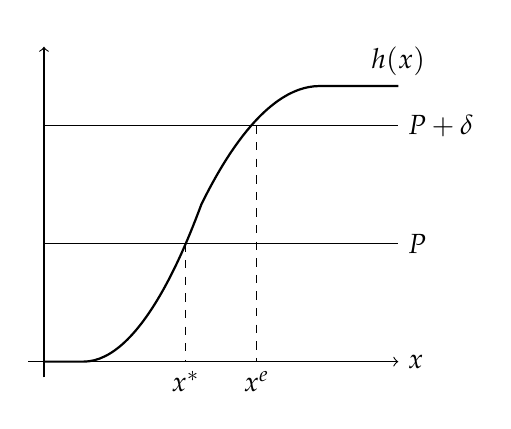
\begin{tikzpicture}[scale=1]
    \draw[->] (-0.2,0) -- (4.5,0) node[right]{$x$}; 
    \draw[->] (0,-0.2) -- (0,4) node[above]{};
    \draw[thick] (0,0) to (0.5,0) parabola (2,2) parabola[bend at end] (3.5,3.5) to (4.5,3.5) node[above]{$h(x)$};
    \draw[thin] (0,1.5) to (4.5,1.5) node[right]{${P}$};
    \draw[dashed, thin] (1.8,1.5) -- (1.8,0) node[below]{$x^*$}; 
    \draw[thin] (0,3) to (4.5,3) node[right]{${P+\delta}$};
    \draw[dashed, thin] (2.7,3) -- (2.7,0) node[below]{$x^e$}; 
\end{tikzpicture}
    \caption{Platform Over-Removal under Strict Liability if $\delta>0$}
    \label{fig:removal}
\end{figure}


\subsection{Imperfect Information and Positive Externality}

The platform is uncertain about whether and to what extent each item is harmful. 
The platform has the prior belief that item $x$ might cause harm $h(x)$ with probability $\lambda(x)\in[0,1]$. Without loss of generality, we assume $\lambda(x)h(x)$ is a weakly increasing function such that the content is ordered by the ascending expected level of harm. We also assume that there is no-harm content ($\lambda(0)=0$) and unambiguously harmful content ($\lambda(1)=1$ and $h(1)=\Bar{h}$).
% And items are heterogeneous in their probability of being harmful. we assume $\lambda(x)$ is a weakly increasing function such that the content is ordered by the ascending likelihood of causing harm.

Given $\hat{x}$, $\int_0^{\hat{x}}\lambda(x)h(x)dx$ is the expected harm given the amount of content $\hat{x}$, and $P\hat{x}$ is the consumer welfare.
The \emph{ex-ante} social welfare function is given by 
\begin{equation}
    \max\{\max_{\hat{x}}P\hat{x}+\delta\hat{x} - \int_0^{\hat{x}}\lambda(x)h(x)dx-F, 0\}.
\end{equation}
Suppose the platform does not shut down, 
the efficient moderation decision $x^e$ is such that
\begin{equation}
    \lambda(x^e)h(x^e)=P+\delta,
\end{equation}
where $P+\delta$ is the marginal social cost of removing the marginal item $x^e$, and $\lambda(x^e)h(x^e)$ is the expected marginal social benefit of removing $x^e$. This is socially efficient if the fixed cost $F$ is not too large.

The analysis can proceed as the last section with the only difference being the expected harm $\lambda(x)h(x)$ instead of the actual harm $h(x)$. Like what we find previously, intermediary immunity is efficient only if the positive externality is sufficiently large. Strict liability lead to over-removal. Negligence based on free speech and safe harbor provision can be efficient. All the liability rules have the same effect except the regime of liability upon notice, which we will elaborate below. 

%% scribe
%% There are going to be two outcomes that are observed here. Outcome one is that this particular item act is harmful. Outcome two, this particular item act is not harmful. 

It is more interesting to consider the environment where the platform can pay an inspection cost $c$ per item to observe a signal of item $x$ indicating whether $x$ is harmful or not. In this case, if the platform chooses to investigate, it can condition its removal decision upon the realization of the signal. The investigation decision will depend upon the cost of investigation and the amount of information the platform gain from it.

%% two alternative ways to solve the problem: 1. mathematical, 2. intuition
Obviously, if the moderation decision remains the same regardless of the realization of the signal, the platform will not incur the cost. 
The signal is useful only if the additional information changes its removal decision. 
Consider content $x\in[0,\hat{x}]$ that will not be removed without investigation. With probability $1-\lambda(x)$ the signal shows no harm and there is no change in the removal decision. With probability $\lambda(x)$ the signal shows harm and this item will be removed. In this case, the marginal value decreases by $P+\delta$ but the marginal harm decreases by $h(x)$, so the net change is $h(x)-P$. This happens with probability $\lambda(x)$, and the expected welfare change is thus $\lambda(x)(h(x)-P-\delta)$.
The social planner prefers the investigation of item $x$ if $\lambda(x)(h(x)-P-\delta)>c$. 
% what we are improving upon it's definitely that you are reducing the harm.

Now consider content $x\in[\hat{x},1]$ that will be removed without investigation. With probability $\lambda(x)$ the signal shows harm and there is no change in the removal decision. With probability $1-\lambda(x)$ the signal shows no harm and this item will not be removed. In either case, the marginal harm $h(x)$ does not show up in the calculation because either the harm has been removed or the investigation finds no harm involved. The benefit of the investigation is to keep the marginal value $P+\delta$ on the platform. The expected welfare change is $(1-\lambda(x))(P+\delta)$. 
The social planner prefers the investigation of item $x$ if $(1-\lambda(x))(P+\delta)>c$. 

Collecting the previous two observations, the social planner wants to pay for the cost only if the welfare improvement exceeds the cost. For $x\ls \hat{x}$, a signal is welfare-improving because it prevents the welfare loss of under-removal. 
%% For $x\ls \hat{x}$, the signal is useful if it reveals the item $x$ is harmful and thus should be removed instead.
Notice that the welfare improvement from under-removal is increasing in $\lambda(x)$.
For $x>\hat{x}$, a signal is welfare-improving because it avoids the welfare loss of over-removal.
Notice that the welfare improvement from over-removal is decreasing in $\lambda(x)$.
% flip the decision

% interval
The next observation is that the platform's investigation decision has to be an interval of items. First notice that there is no value in investigating the no-harm content or the unambiguously harmful content; it is the more ambiguous content in between that provides an incentive for investigation. 
%% And the second observation is that if you want to investigate, it has to be the fact that the lambda has to have a sufficient amount of uncertainty there such that it's beneficial for us to investigate. 
Because of the monotonicity of $\lambda(x)h(x)$, it is suboptimal to pick two disconnected sets and have a gap in between. The platform is always better to join the two sets and leave the less ambiguous items at the ends while keeping the total investigation cost constant. Therefore choosing an interval is a dominant strategy of investigation. 

% now the problem is how to choose the interval
The final step is to determine the optimal choice of the interval. 
An interval is characterized by two parameters: the lower range $\underline{x}$ and the upper range $\overline{x}$. The social planner's problem is as follows:
\begin{equation}
    \max_{\underline{x},\overline{x}} \int_{\underline{x}}^{\overline{x}} [(1-\lambda(x))(P+\delta)-c]dx + \int_0^{\underline{x}} [P+\delta-\lambda(x)h(x)]dx 
\end{equation}
Note that the interval must contain $\hat{x}$ (the moderation decision without investigation). Otherwise, the interval will either contain $x=0$ or $x=1$ leading to a contradiction. 
The lower range $\underline{x}^e$ is determined by the indifference condition of investigating to avoid under-removal (i.e., flip a non-removal decision to a removal decision) such that $\lambda(\underline{x}^e)(h(\underline{x}^e)-P-\delta)=c$. At $\underline{x}^e$, the social planner is just indifferent between paying the cost and the welfare improvement from under-removal. 
The upper range $\overline{x}^e$ is determined by the indifference condition of investigating to avoid over-removal (i.e., flip a removal decision to a non-removal decision) such that $(1-\lambda(\overline{x}^e))(P+\delta)=c$. 

The efficient moderation outcome is to (i) carry $[0,\underline{x}^e)$ and remove $(\overline{x}^e,1]$ without investigation, and (ii) investigate $[\underline{x}^e,\overline{x}^e]$ and remove if it is found harmful and carry otherwise.  
The efficient investigation decision varies with the cost $c$. If $c=0$ such that investigation is costless, the optimal interval is $[0,1]$ that covers the entire content spectrum. As $c$ grows, the interval shrinks until it does not make sense to investigate at all (i.e., $c\ls\frac{P(h(x^e)-P)}{h(x^e)}$, a sufficient condition is $c\ls\frac{P\delta}{P+\delta}$). When $c$ is sufficiently large, we are back in an environment as if no investigation technology is available.


\textbf{Intermediary immunity}.
Because the platform faces no liability for any harm, it does not have any incentive to investigate the harm. It will not pay for the signal as it will carry all the content regardless of the harm. Compared with the social optimum, immunity leads the platform to under-investigate and under-remove. 

\textbf{Strict liability}.
Under strict liability, the platform's investigation problem becomes 
\begin{equation}
    \max_{\underline{x},\overline{x}} \int_{\underline{x}}^{\overline{x}} [(1-\lambda(x))P-c]dx + \int_0^{\underline{x}} [P-\lambda(x)h(x)]dx 
\end{equation}
Note that the platform does not take the positive externality into account, and in calculating the investigation trade-off it only cares about the change in the marginal revenue $P$ (as opposed to $P+\delta$). 
% the idea that you've seen the removal part, but now in the investigation world, you still want to have the same set that the marginal benefit of your investigation covers your cost of the investigation.
% All the stars are for the platform, all the e are for the efficiency. that's why you see in this graph, c is showing up for every single line.
Figure 6 extends figure 5 and compares the socially optimal investigation with the platform's investigation under strict liability. The platform's investigation decision is $[\underline{x}^*,\overline{x}^*]$ where the lower range and the upper range are identified by the intersection of $\lambda(x)$ and the two lines of marginal private cost $\frac{c}{h-P}$ and $1-\frac{c}{P}$. 
In contrast, the lower range and the upper range required by efficiency are located at the intersection of $\lambda(x)$ and the two lines of marginal social cost $\frac{c}{h-(P+\delta)}$ and $1-\frac{c}{P+\delta}$.  
We observe that the platform's interval is always lower than the efficient interval. The decision to investigate $[\underline{x}^e,\overline{x}^*]$ is efficient, but the deicision to investigate $[\underline{x}^*,\underline{x}^e]$ as opposed to $[\overline{x}^*,\overline{x}^e]$ is inefficient. In this sense, we say the platform is biased in investigation under strict liability. Strict liability leads the platform to investigate the \emph{wrong} types. This happens because the platform cannot internalize the positive externality of the content. The consequence of under-investigation is over-removal. The platform is doing uninformed removal of the upper tail $[\overline{x}^*,\overline{x}^e]$, and is having excessive scrutiny over the lower tail $[\underline{x}^*,\underline{x}^e]$. As a result, the platform is carrying too little content.

% platform make blunter decisions to take down too much content at the lower end of the range or to leave up too much content at the upper end of the range. 

\begin{figure}[h]
    \centering
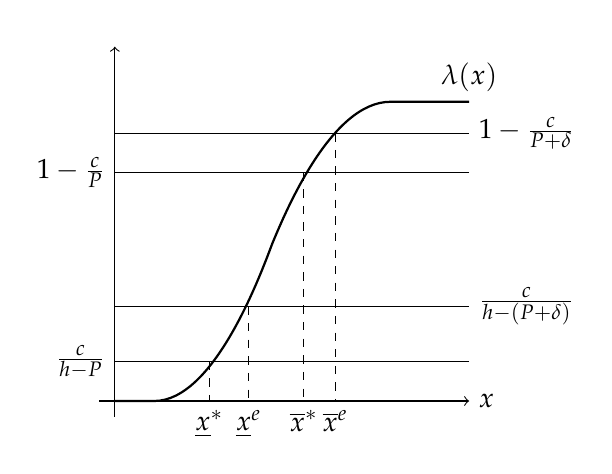
\begin{tikzpicture}[scale=1]
    \draw[->] (-0.2,0) -- (4.5,0) node[right]{$x$}; 
    \draw[->] (0,-0.2) -- (0,4.5) node[above]{};
    \draw[thick] (0,0) to (0.5,0) parabola (2,2) parabola[bend at end] (3.5,3.8) to (4.5,3.8) node[above]{$\lambda(x)$};
    %% next four \draw are efficiency
    \draw[thin] (0,1.2) to (4.5,1.2) node[right]{$\frac{c}{h-(P+\delta)}$};
    \draw[thin] (0,3.4) to (4.5,3.4) node[right]{$1-\frac{c}{P+\delta}$};
    \draw[dashed, thin] (1.7,1.2) -- (1.7,0) node[below]{$\underline{x}^e$};
    \draw[dashed, thin] (2.8,3.4) -- (2.8,0) node[below]{$\overline{x}^e$};
    %% next four \draw are profit
    \draw[thin] (4.5,0.5) to (0,0.5) node[left]{$\frac{c}{h-P}$}; 
    \draw[thin] (4.5,2.9) to (0,2.9) node[left]{$1-\frac{c}{P}$};
    \draw[dashed, thin] (1.2,0.5) -- (1.2,0) node[below]{$\underline{x}^{\ast}$};
    \draw[dashed, thin] (2.4,2.9) -- (2.4,0) node[below]{$\overline{x}^{\ast}$};   
\end{tikzpicture}
    \caption{Biased Investigation of the Platform under Strict Liability if $\delta>0$}
    \label{fig:investigation}
\end{figure}


\textbf{Free speech law}.
Notice that $\underline{x}^e$ has two roles in the efficient solution: it is the lower bound for investigation, \emph{and} the upper bound for removal without investigation. It is a natural threshold for the reasonable person standard in this environment. The negligence rule is thus
\begin{equation}
d(x)=
\lt\{\begin{array}{ll}
    h(x) & \mbox{if $x$ is not removed and $x\in[\underline{x}^e,1]$}, \\ % part of x
    0 & \mbox{otherwise}.
\end{array}\rt.
\end{equation}
The free speech region is $[0,\underline{x}^e]$ where carrying any content leads to no liability and the negligence region is $[\underline{x}^e,1]$ where carrying any content leads to strict liability. 
Platform's problem under this rule is 
\begin{equation}
    \max_{\underline{x},\overline{x}} \int_{\underline{x}}^{\overline{x}} [(1-\lambda(x))P-c]dx + \int_0^{\underline{x}} [P-\lambda(x)h(x)I(x\in[\underline{x}^e,1])]dx 
\end{equation}
This takes into account the fact that if the investigation interval overlaps with the negligence region, the platform will remove the content to avoid liability. First, notice that $\underline{x}$ is at least $\underline{x}^e$ otherwise it contradicts profit maximization. Next notice that the marginal revenue of moving just above $\underline{x}^e$ is negative as $\lambda(\underline{x}^e)[P-h(\underline{x}^e)]+c=-\lambda(\underline{x}^e)\delta<0$. Thus $\underline{x}$ is at most $\underline{x}^e$ and it follows that $\underline{x}^*=\underline{x}^e$. The lower range choice is efficient under the free speech law. The upper range choice, however, will not be efficient. The platform will choose $\overline{x}^*$ such that $(1-\lambda(\overline{x}^*))P=c$. As $[\underline{x}^*,\overline{x}^*]\subset[\underline{x}^e,\overline{x}^e]$, The platform shirks its effort on investigation, and the inefficiency problem is under-investigation.  


\textbf{Safe harbor provision}.
Defining a standard for total harm is not obvious here. There are two choices we can consider: \emph{ex-ante} total harm and \emph{ex-post} total harm.
Setting the standard on \emph{ex-post} total harm is hard to monitor. Suppose the rule is conditional on the investigation such that if the platform finds the content harmful, failure to remove it will result in liability. It actually provides the platform with disincentive to find out about the content in the first place.  

% revisit the efficient objective
A safe harbor provision that caps the \emph{ex-ante} total harm can be formulated as follows:
\begin{equation}
d(x)=
\lt\{\begin{array}{ll}
    h(x) & \mbox{if $\int_0^{\underline{x}}\lambda(x)h(x)dx>s_h=\int_0^{\underline{x}^e}\lambda(x)h(x)dx$}, \\
    0 & \mbox{otherwise}.
\end{array}\rt.
\end{equation}
Suppose the platform chooses $\underline{x}>\underline{x}^e$ such that it loses the safe harbor status, the penalty in liability would be $\int_0^{\underline{x}}\lambda(x)h(x)dx$ whereas the gain in revenue would be $\int_{\underline{x}^e}^{\underline{x}}[\lambda(x)P+c]$. The deviation is not profitable.
The optimal choice $\underline{x}^*$ is equal to $\underline{x}^e$ such that the platform maximizes the profits without losing its safe harbor status. 
\footnote{It is sub-optimal to carry items of higher types while keeping the total harm constant, which results in less content and thus less revenue.}

For $x>\underline{x}$, the platform wants to carry as much content as possible but fears going beyond the safe harbor limit. The platform has an incentive to investigate to keep the safe harbor status. It will do so until the marginal expected revenue $(1-\lambda(x))P$ can no longer justify the investigation cost $c$. The upper range $\overline{x}^*$ is such that $(1-\lambda(\overline{x}^*))=c$. 
Since $\overline{x}^*<\overline{x}^e$, platform under-investigate.
Setting the standard on total harm alone does not provide sufficient incentive for investigation.

However, a safe harbor provision may not only be conditioned on the total harm, but can also be conditioned on other observables. And in fact, a safe harbor provision directly regulating the investigation effort can lead to the efficient moderation outcome. A safe harbor provision, that both caps the total harm and requires a floor on total investigation cost, is characterized by a pair of standards $(s_h,s_c)$ such that:
\begin{equation}
d(x)=
\lt\{\begin{array}{ll}
    0 & \mbox{if $\int_0^{\underline{x}}\lambda(x)h(x)dx\ls s_h$ and $c[\overline{x}-\underline{x}]\gs s_c$}, \\
    h(x) & \mbox{otherwise}.
\end{array}\rt.
\end{equation}
We know from our previous discussion that the platform prefers to keep the safe harbor status. Because of the requirement of minimal effort, the platform would investigate at least up to the efficient upper bound such that $\overline{x}^*\gs\overline{x}^e$. Will the platform investigate more than necessary ? It will not. As the profit change at $\overline{x}^e$ is negative, i.e., $(1-\lambda(\overline{x}^e))P-c=-(1-\lambda(\overline{x}^e))\delta<0$.  

Therefore, we can formulate the platform's problem as profit maximization subject to two policy constraints:
\begin{eqnarray}
\max_{\underline{x},\overline{x}} &&
\hspace{-1em} P\underline{x}+\int_{\underline{x}}^{\overline{x}} [(1-\lambda(x))P-c]dx \nn\\
\mbox{s.t.} &&\hspace{-1em} \int_0^{\underline{x}}\lambda(x)h(x)dx\ls s_h, \nn\\
&&\hspace{-1em} c[\overline{x}-\underline{x}]\gs s_c.
\end{eqnarray}
If the pair of threshold is chosen properly such that $s_h=\int_0^{\underline{x}^e}\lambda(x)h(x)dx$ and $s_c=c[\overline{x}^e-\underline{x}^e]$. 
The two constraints are binding such that $\underline{x}^*=\underline{x}^e$ and $\overline{x}^*=\overline{x}^e$.
Safe harbor provision leads to the efficient moderation outcome.


\textbf{Liability Upon Notice}.
%% platform's strategy is not an interval
%% this should be a PBE; users may not be truthful?
The notice serves the same function as a signal that tells the platform whether the item in question is harmful or not. In that sense, liability upon notice shifts the cost of investigation to the harmed parties.
We will start with the assumption that the platform does not investigate in addition to the notices. The platform's decision would be a threshold denoted by $\underline{x}^*$. Equivalently for comparison, we can also think of the platform choosing an interval $[\underline{x}^*,1]$. We will then relax this assumption and allow the platform to investigate. We will see that the platform has no incentive to do extra investigations. 

Users, being completely informed, will send a notice if and only if $h(x)\gs c$. 
For items $x\in[0,h^{-1}(c))$, the platform is not liable for any harm, thus $\underline{x}^*$ is at least $h^{-1}(c)$. For items $x\in[h^{-1}(c),1]$, there is a probability $1-\lambda(x)$ that no notice is received and if that happens, the platform will carry the content. There is a probability $\lambda(x)$ that the platform receives a notice, in which case it will remove $x$ if $P<h(x)$. If $P\ls c$, every notice leads to a takedown. If instead $P>c$, some notices do not lead to a takedown, and $h(\underline{x}^*)=P$. Thus in this sequential move game, the platform will set $\underline{x}^*$ such that $h(\underline{x}^*)=\max\{P,c\}$. Suppose we allow the platform to investigate, it is easy to show that it is not profitable to investigate any item $x\in[0,h^{-1}(c))$.

The welfare implied by the platform's decision and the users' notice choice can be evaluated from the social planner's \emph{ex-ante} perspective:
\begin{equation}
(P+\delta)\underline{x}^*+\int_{\underline{x}^*}^1 (1-\lambda(x))(P+\delta)dx-\int_{h^{-1}(c)}^{\max\{\underline{x}^*,h^{-1}(c)\}}\lambda(x)h(x)dx-\int_{h^{-1}(c)}^{1}\lambda(x)cdx
\end{equation}
Compared with the efficiency solution, notice that $h(\underline{x}^*)=\max\{P,c\}<P+\delta+\frac{c}{\lambda(\underline{x}^e)}=h(\underline{x}^e)$. It follows that $\underline{x}^*<\underline{x}^e$ and $[\underline{x}^e,\overline{x}^e]\subset[\underline{x}^*,1]$. 
Liability upon notice is not efficient even though it saves the platform's cost of acquiring information. 
The inefficiency comes from the fact that the notice procedure is over-used, and too many notices lead the platform to carry too little content.





%% The platform receives a revenue of $R \ge 0$ for each item it carries, good or bad. It can tell the difference between the two types at a cost of $C \ge 0$ per item. If it decides to remove an item of content, it gives up the revenue associated with that item.

% Putting this all together, the case for intermediary immunity is justified when $C > C^*$ and $\beta < G/(B+G)$ (one paragraph explains C*, one explain C>C*, one explain second inequality) Effective filtering is cost-prohibitive, so that imposing liability will lead the platform to overfilter (from society's point of view) by shutting down. But since society prefers to have the platform to not having it (because the good content still outweighs the bad), it is better off with underfiltering than overfiltering.


%must carry or must remove rule
%Must remove rule
% Q. loss of safe harbor means all the content is liable for $d$, or only part of the content liable for $d$.

%(i) If all the platform can do is content removal and no positive externality, strict liability leads to efficiency.
%(ii) content removal + positive externality, strict liability leads to over-removal and immunity might be justified if the externality is sufficiently large (though that means keeping all the content).
%(iii) If platform can first choose whether to investigate and then decide on removal, with no positive externality, strict liability again leads to efficiency !
%(iv) investigate + removal + positive externality, strict liability leads to under-investigation and over-removal.  
%(v) imperfect signal does not change (iii) and (iv). 

% (iii)For complete info+no externality, (b)(c)(d)(e) can all lead to efficient outcome.
% (iv)For complete info+positive externality, (a) can be efficient under some condition. (b)(e) lead to over-removal. (c)(d) lead to efficient outcome.
% v) For incomplete info+positive externality, (a)(b)(c)(e) are all sub-optimal. There might be some version of (d) that leads to efficient outcome (I'm still figuring that out).

In conclusion, many liability rules fail in this rich environment where content has positive externality, the platform has imperfect information regarding the harm, information can be transmitted either through investigation or through notices. Immunity, strict liability, free speech, and liability upon notice are all inefficient. The only efficient rule is a safe harbor provision based on total harm and reasonable effort.

\begin{proposition}
Given imperfect information and positive externality, a safe harbor provision, which both caps the total harm and requires a minimal effort on investigation, leads to the efficient moderation outcome. 
\end{proposition}

%\section{Extensions}\label{EMIL_Section:ext}
%






\subsection{Inelastic Demand}
In the last section, we assume that all content is \emph{ex-ante} homogeneous. We relax that assumption in this section.
There are two types of content $\{G, B\}$ where $G$ stands for the good content, and $B$ stands for the bad content. Let $\lambda$ be the proportion of type $B$ content. The total amount of type $G$ content and type $B$ content are then $(1-\lambda)x$ and $\lambda x$ respectively. 

Suppose a perfect filter is available such that the moderation will remove all the type $B$ content. Social welfare from moderation is $\int_0^{(1-\lambda)x} P(z)dz-1$. Social welfare without moderation is $\int_0^x P(z)dz-\lambda xh$. A social planner prefers moderation if 
\begin{equation}\label{eqn:efficiency_2}
    \lambda xh - \int_{(1-\lambda)x}^x P(z)dz \gs 1,
\end{equation}
where $\lambda xh$ is the expected harm, $\int_{(1-\lambda)x}^x P(z)dz$ is the loss of total surplus because of the reduction in content, and $1$ is the marginal cost of moderation.

The platform's profit from moderation is $P((1-\lambda)x)(1-\lambda)x-1$. The profit with no moderation is $P(x)x-\lambda xd$. The platform prefers moderation if 
\begin{equation}\label{eqn:platform_2}
    \lambda xd - [P(x)x-P((1-\lambda)x)(1-\lambda)x] \gs 1,
\end{equation}
where $P(x)x-P((1-\lambda)x)(1-\lambda)x$ is the change in profits because of the reduction in content. 

Notice that the loss in profit is always smaller than the loss in total surplus since 
\begin{equation*}
    P(x)x-P((1-\lambda)x)(1-\lambda)x \ls P((1-\lambda)x)\lambda x \ls \int_{(1-\lambda)x}^x P(z)dz.
\end{equation*}
Therefore, $d<h$ so that the strict liability is \emph{never} optimal. If $d=h$, the platform will more likely to moderate than desired. 
The optimal liability can be written as 
\begin{equation}\label{eqn:liability_1}
    d=\min \left\{h-\frac{\int_{(1-\lambda)x}^x [P(z)-\hat{P}]dz}{\lambda x}, 0\right\},
\end{equation}
which is the harm minus the normalized per-item loss in consumer surplus conditional on the quantity is non-negative. 

When, if ever, will platform immunity $d=0$ be optimal ? It must be that the first part of equation \ref{eqn:liability_1} is less or equal to zero. And observe that 
\begin{equation*}
    \lambda xh < \int_{(1-\lambda)x}^x [P(z)-\hat{P}]dz < \int_{(1-\lambda)x}^x P(z)dz + 1.
\end{equation*}
Hence, it must be that efficiency requires no moderation. This will be true under one of the two conditions: either (i) the harm $h$ is small, or (ii) the fraction of problematic content $\lambda$ is neither too small nor too large. 

Intuitively, moderation is not socially optimal if the harm is too small or the number of problematic item is too few such that the marginal social benefit cannot justify the cost. Interestingly, when the platform is overwhelmed with problematic content while each of them generates negligible harm, moderation is also sub-optimal because moderation in that case virtually means shutting down a platform with positive consumer welfare (Napster is arguably one such case). 
To see the second point more clearly, the first order derivative of the marginal social benefit (on the left-hand side of equation \ref{eqn:efficiency_2}) with respect to $\lambda$ is $x[h-P((1-\lambda)x)]$, which is positive if $P((1-\lambda)x)<h$ and negative if $P((1-\lambda)x)\gs h$. It follows that as $\lambda$ increases, the social benefit of moderation first goes up and above $1$, reaches its peak, and then goes down and below $1$. 

%%% Adding a graph, regions of liability


\subsection{Imperfect Filter and Investment in Filter}
% (3) Platform can invest to create a better filter

The analysis in the last section assumed no ``false positives''. That is, the moderation technology does not erroneously remove type $G$ content and keep type $B$ content. In reality, such errors happened all the time.\footnote{There are accumulating evidence on over-removal of content by mistakes. See for example, \url{https://cyberlaw.stanford.edu/blog/2021/02/empirical-evidence-over-removal-internet-companies-under-intermediary-liability-laws}}

Let $\pi(s)\in [\frac{1}{2},1]$ be the accuracy of the filter given the expenditure on moderation $s$. If an item is of type $B$, it will be removed with probability $\pi(s)$ and kept with probability $1-\pi(s)$. If an item is of type $G$, it will be kept with probability $\pi(s)$ and removed with probability $1-\pi(s)$. As a consequence, the remaining type-$G$ content after moderation is $\pi(s)(1-\lambda)x$ and the remaining type-$B$ content is $(1-\pi(s))\lambda x$. The expected harm is then $(1-\pi(s))\lambda xh$.



\subsection{User submitted content}
$\lambda(x)$ is endogenous

%\section{Conclusion}\label{EMIL_Section:conclude}
%\input{./EMIL_tex/S5_Conclusion.tex}

\newpage
\appendix
%\input{./EMIL_tex/S6_AppendixA.tex}\label{Appendix:proofs}


\end{document}




